\documentclass[bachelor, fontsize=14pt]{diploma}

\usepackage{booktabs}

\providecommand{\tightlist}{%
  \setlength{\itemsep}{0pt}\setlength{\parskip}{0pt}%
}
\providecommand{\passthrough}[1]{#1}

% TODO: заменить плейсхолдеры на реальные данные перед финальной сдачей.
\student{ФИО студента}
\group{Группа}
\theme{Создание открытой микросервисной платформы для автоматизации тренировочного процесса и взаимодействия в системе <<тренер-спортсмен>>}

\supervisor{ФИО руководителя}
\firstConsultant{}
\secondConsultant{}
\reviewer{}

\faculty{№ 8 <<Компьютерные науки и прикладная математика>>}
\department{806}
\speciality{01.03.02 <<Прикладная математика и информатика>>}
\profile{Информатика}

\departmentFullName{№ 806}
\headOfDepartment{ФИО заведующего кафедрой}

% Дата. Оставляем пустое место для дня
\date{\uline{\hspace{24pt}} мая \the\year\ года}

\newacronym{api}{API}{Application Programming Interface, программный интерфейс приложения}
\newacronym{rest}{REST}{Representational State Transfer, архитектурный стиль построения HTTP API}
\newacronym{jwt}{JWT}{JSON Web Token, формат токена для передачи утверждений о пользователе}
\newacronym{fcm}{FCM}{Firebase Cloud Messaging, сервис push-уведомлений}
\newacronym{llm}{LLM}{Large Language Model, большая языковая модель}
\newacronym{rpe}{RPE}{Rate of Perceived Exertion, субъективная оценка тяжести нагрузки}
\newacronym{db}{БД}{база данных}


\newglossaryentry{backend}{
    name={Backend},
    description={серверная часть программной системы, отвечающая за бизнес-логику, хранение данных, API и межсервисное взаимодействие}
}

\newglossaryentry{microservice}{
    name={Микросервис},
    description={независимый сервис, реализующий ограниченную область ответственности и взаимодействующий с другими сервисами через API или сообщения}
}

\newglossaryentry{api-gateway}{
    name={API Gateway},
    description={сервис, выступающий единой точкой входа для внешних клиентов и маршрутизирующий запросы к внутренним backend-сервисам}
}

\newglossaryentry{training-plan}{
    name={Тренировочный план},
    description={описание задания, сформированного тренером для одного или нескольких спортсменов}
}

\newglossaryentry{training-report}{
    name={Тренировочный отчет},
    description={структурированная обратная связь спортсмена о выполненной тренировке}
}

\newglossaryentry{event-driven}{
    name={Событийное взаимодействие},
    description={способ обмена данными между сервисами, при котором один сервис публикует событие, а другие сервисы обрабатывают его асинхронно}
}

\newglossaryentry{stateless}{
    name={Stateless-сервис},
    description={сервис, не владеющий собственным состоянием предметной области и вычисляющий результат на основе входных данных или данных других сервисов}
}



\addbibresource{main.bib}

\begin{document}
    \maketitle

    % \includepdf[pages=-]{extra/task} % Задание на ВКР при необходимости
    \setcounter{page}{2}

    \abstract

\keywords{BACKEND-ПЛАТФОРМА, МИКРОСЕРВИСНАЯ АРХИТЕКТУРА, ТРЕНЕР, СПОРТСМЕН, ТРЕНИРОВОЧНЫЙ ПРОЦЕСС, REST API, NATS JETSTREAM, POSTGRESQL, АНАЛИТИКА, AI-РЕКОМЕНДАЦИИ}

Выпускная квалификационная работа посвящена разработке backend-части открытой микросервисной платформы CoachLink для автоматизации тренировочного процесса и взаимодействия в системе <<тренер-спортсмен>>. В работе рассматривается проблема разрозненного обмена тренировочными заданиями и отчётами через мессенджеры, электронные таблицы и произвольные форматы данных.

Объектом исследования является процесс информационного взаимодействия между тренером и спортсменом при планировании, выполнении и анализе тренировок. Предметом исследования является backend-платформа для автоматизации назначения тренировочных заданий, сбора стандартизированных отчётов, отправки уведомлений и анализа данных тренировочного процесса.

Целью работы является разработка backend-части открытой микросервисной платформы для автоматизации тренировочного процесса и взаимодействия в системе <<тренер-спортсмен>>.

В рамках работы спроектирована и реализована микросервисная архитектура из семи независимых сервисов. Сервисы реализованы на языке Go, используют PostgreSQL для хранения данных, NATS JetStream для событийного взаимодействия и OpenAPI для документирования публичных интерфейсов. Backend обеспечивает регистрацию пользователей, разграничение ролей тренера и спортсмена, управление связями и тренировочными группами, назначение тренировок, приём стандартизированных отчётов, формирование уведомлений, агрегацию тренировочных данных и генерацию AI-рекомендаций на основе истории тренировок.

Первая версия ориентирована на лёгкую атлетику, однако архитектура позволяет адаптировать тренировки, отчёты и шаблоны под другие виды спорта.


    \tableofcontents
    \termsanddefenitions
    \listofabbreviations

    \introduction

Современный тренировочный процесс всё чаще опирается не только на очное взаимодействие тренера и спортсмена, но и на постоянный обмен цифровыми данными. Тренер должен заранее формировать тренировочные задания, распределять их между спортсменами, учитывать индивидуальные особенности подготовки, получать обратную связь после выполнения тренировки и принимать решения о дальнейшем изменении нагрузки. При работе с одним спортсменом такие действия могут выполняться вручную и не требуют сложной информационной системы. Однако при увеличении количества спортсменов и появлении тренировочных групп ручной обмен сообщениями быстро становится неудобным и ненадёжным.

На практике взаимодействие тренера со спортсменами часто организуется с помощью мессенджеров, электронных таблиц и произвольных файлов. Такой подход не требует внедрения специализированного программного обеспечения, но создаёт ряд существенных проблем, подробно рассмотренных в первой главе. Особенно остро они проявляются в циклических видах спорта, где важно не только получить отдельный отчёт, но и накопить историю структурированных данных для оценки динамики подготовки.

В связи с этим актуальной является задача разработки единой backend-платформы, которая автоматизирует взаимодействие тренера и спортсмена, стандартизирует формат тренировочных отчётов, обеспечивает хранение истории тренировок и предоставляет программные интерфейсы для внешних клиентских приложений. Такая платформа должна решать не только задачу обмена сообщениями, но и задачу организации предметной логики тренировочного процесса: ролей пользователей, связей между тренером и спортсменами, групп, планов, назначений, отчётов, уведомлений и аналитики.

В данной работе рассматривается backend-часть платформы CoachLink. Backend реализует серверную логику, хранение данных, публичные REST API, межсервисное взаимодействие и интеграцию с инфраструктурными компонентами. Мобильное приложение рассматривается только как внешний клиент, который обращается к backend через API Gateway. Разработка мобильного приложения не входит в область ответственности данной выпускной квалификационной работы.

Платформа CoachLink проектируется как расширяемая система для автоматизации тренировочного процесса в различных видах спорта. В целях упрощения разработки прототипа текущая реализация ориентирована исключительно на лёгкую атлетику. При этом архитектура платформы остаётся универсальной: базовые сущности (пользователь, тренер, спортсмен, группа, план, назначение, отчёт, уведомление) не имеют жёсткой привязки к конкретному виду спорта и в дальнейшем могут быть расширены за счёт добавления специфических атрибутов и шаблонов для других дисциплин.

Объектом исследования является процесс информационного взаимодействия между тренером и спортсменом при планировании, выполнении и анализе тренировок.

Предметом исследования является backend-платформа для автоматизации назначения тренировочных заданий, сбора стандартизированных отчётов, отправки уведомлений и анализа данных тренировочного процесса.

Целью выпускной квалификационной работы является разработка открытой микросервисной backend-платформы CoachLink для стандартизации и автоматизации взаимодействия в системе «тренер-спортсмен».

Для достижения поставленной цели необходимо решить следующие задачи:

\begin{enumerate}
\def\labelenumi{\arabic{enumi}.}
\tightlist
\item
  провести анализ предметной области и существующих программных решений, выявить их ограничения в контексте автоматизации взаимодействия тренера и спортсмена;
\item
  сформулировать функциональные и нефункциональные требования к backend-платформе;
\item
  спроектировать микросервисную архитектуру системы, разработать модель данных и спецификации программных интерфейсов;
\item
  реализовать спроектированные микросервисы и обеспечить их взаимодействие;
\item
  провести тестирование backend-компонентов и оценить соответствие разработанной системы исходным требованиям.
\end{enumerate}

При выполнении работы используются методы системного анализа, объектно-ориентированного и компонентного проектирования, проектирования REST API, проектирования реляционных баз данных и тестирования программного обеспечения. Выбор микросервисной архитектуры соотносится с подходами к построению распределённых систем, описанными в работах по шаблонам микросервисов, проектированию независимых сервисов и переходу к cloud-native архитектурам~\cite{richardson-microservices,newman-microservices-2021,dragoni-microservices,balalaie-microservices-devops}.

Теоретическая значимость работы заключается в проектировании модели backend-платформы, объединяющей микросервисный подход, событийное взаимодействие, стандартизированный сбор тренировочных данных и аналитическую обработку этих данных. Работа демонстрирует, как предметная область тренировочного процесса может быть представлена через набор независимых сервисов с чёткими зонами ответственности.

Практическая значимость заключается в создании открытой серверной основы для платформы CoachLink. Реализованный backend может использоваться как база для дальнейшего развития системы: подключения мобильного приложения, добавления новых видов спорта, расширения аналитики, интеграции со спортивными устройствами и развития AI-сценариев. Благодаря открытому API систему можно адаптировать под разные клиентские приложения и внешние интеграции.

Выпускная квалификационная работа состоит из введения, трёх глав, заключения и приложений.

В первой главе проводится аналитический обзор существующих подходов к организации взаимодействия тренера и спортсмена. Рассматриваются мессенджеры, электронные таблицы, спортивные трекеры и специализированные коммерческие платформы. На основе сравнения формулируются требования к backend-платформе.

Во второй главе описывается проектирование CoachLink. Рассматриваются архитектура микросервисов, модель данных, межсервисное взаимодействие, ключевые пользовательские сценарии и выбор технологического стека.

В третьей главе описывается практическая реализация спроектированных микросервисов и результаты тестирования.

В заключении подводятся итоги работы, оценивается достижение цели и формулируются направления дальнейшего развития платформы.

    \section{АНАЛИТИЧЕСКИЙ ОБЗОР}

\subsection{Особенности взаимодействия тренера и спортсмена}

Тренировочный процесс представляет собой повторяющийся цикл планирования, выполнения, отчётности и корректировки нагрузки. Тренер формирует задание, спортсмен выполняет его и передаёт обратную связь, после чего тренер оценивает состояние спортсмена и принимает решение о следующем этапе подготовки. Для эффективной работы важно, чтобы этот цикл был регулярным, прозрачным и основанным на достоверных данных.

В классической форме взаимодействие тренера и спортсмена может происходить очно: тренер объясняет задание на тренировке, наблюдает за выполнением и сразу корректирует действия спортсмена. Однако в реальных условиях такая модель не всегда достаточна. Спортсмены могут выполнять часть тренировок самостоятельно, находиться в разных местах, тренироваться в разное время или входить в разные группы. Поэтому тренеру необходим цифровой инструмент, позволяющий сопровождать тренировочный процесс вне очных занятий.

Цифровая поддержка тренировочного процесса должна решать несколько задач:

\begin{enumerate}
\def\labelenumi{\arabic{enumi}.}
\tightlist
\item
  передача тренировочных заданий спортсменам;
\item
  управление индивидуальными и групповыми назначениями;
\item
  получение отчётов о выполнении заданий;
\item
  хранение истории тренировок;
\item
  уведомление участников о важных событиях;
\item
  анализ накопленных данных;
\item
  разграничение ролей и прав доступа.
\end{enumerate}

Если рассматривать систему только как средство отправки сообщений, можно ограничиться мессенджером. Но при необходимости хранить историю тренировок, связывать отчёт с конкретным заданием и выполнять аналитику простого обмена сообщениями становится недостаточно. Требуется система, в которой данные имеют заранее определённую структуру.

\subsection{Использование мессенджеров}

Мессенджеры выступают наиболее распространённым инструментом цифрового взаимодействия благодаря своей массовости и интуитивно понятному интерфейсу, не требующему времени на освоение. Данный класс приложений позволяет тренеру оперативно создавать групповые чаты, рассылать тренировочные задания или консультировать спортсменов в индивидуальном порядке. В свою очередь, спортсмен получает возможность быстро предоставлять обратную связь, используя различные форматы данных.

Главное преимущество мессенджеров --- низкий порог входа. Для начала работы не требуется разрабатывать отдельную систему, создавать аккаунты в специализированном сервисе или обучать пользователей. Мессенджер удобен для оперативного общения и решения организационных вопросов.

Однако при использовании мессенджеров для ведения тренировочного процесса возникают существенные ограничения.

Ключевым ограничением является отсутствие стандартизированной структуры отчёта: спортсмен сам решает, что написать и в каком формате, в результате чего тренер получает разноформатные данные, непригодные для автоматической обработки.

Помимо этого, отчёты трудно связывать с конкретными заданиями. Если спортсмен прислал сообщение спустя несколько дней после нескольких назначений, тренер вынужден вручную восстанавливать соответствие, что особенно неудобно при групповой работе.

Существенной проблемой остаётся смешение тренировочных данных с общей перепиской: организационные сообщения, личные вопросы и отчёты оказываются в одном чате, что затрудняет поиск и систематизацию истории тренировок.

Наконец, мессенджеры не предоставляют аналитических инструментов: рассчитать процент выполнения заданий, динамику нагрузки или суммарную дистанцию без ручной обработки данных невозможно.

Следовательно, мессенджер эффективен как канал общения, но не является полноценной платформой для управления тренировочным процессом.

\subsection{Использование электронных таблиц}

Электронные таблицы частично решают проблему структуры данных. Тренер может создать таблицу с колонками для даты, задания, длительности, дистанции, пульса и комментария. Спортсмены могут заполнять строки после выполнения тренировок, а тренер --- просматривать данные и выполнять простые расчёты.

Преимущество таблиц заключается в том, что они позволяют хранить историю тренировок в более структурированном виде, чем мессенджеры. Таблицы также поддерживают фильтрацию, сортировку, формулы и визуализацию. Для небольших групп этого может быть достаточно.

Однако у таблиц также есть ограничения.

Ключевым ограничением является отсутствие полноценной ролевой модели: доступ можно настроить лишь на уровне документа или листа, но выразить предметные правила --- кто видит только свои задания, кто видит всю группу --- средствами таблицы затруднительно.

Вместе с тем таблицы не моделируют жизненный цикл задания: они хранят данные, но не отражают переходы между состояниями «назначено», «выполнено», «в архиве», что делает контроль за выполнением непрозрачным.

Дополнительную сложность создаёт отсутствие встроенного механизма уведомлений: тренер не получает системного оповещения об отправленном отчёте, а спортсмен может не заметить новое задание без дополнительного сообщения в мессенджере.

Наконец, при росте числа спортсменов таблица становится трудноуправляемой: возникает риск случайного изменения чужих данных, удаления строк и нарушения согласованности формата.

Таким образом, электронные таблицы лучше мессенджеров подходят для хранения истории, но не обеспечивают полноценную автоматизацию взаимодействия.

\subsection{Спортивные трекеры и приложения}

Спортивные трекеры и приложения предназначены для фиксации фактических показателей активности. Они могут автоматически собирать дистанцию, темп, пульс, маршрут, высоту, каденс и другие параметры. Для лёгкой атлетики такие инструменты полезны, потому что позволяют получить объективные данные о тренировке.

Сильной стороной спортивных трекеров является автоматизация измерений. Спортсмену не нужно вручную вводить все показатели, если устройство уже записало тренировку. Также многие приложения предоставляют графики и базовую аналитику.

Однако спортивные трекеры не полностью решают задачу взаимодействия тренера и спортсмена.

Ключевым ограничением является ориентированность трекеров на фиксацию факта активности, а не на управление назначениями: логика «задание назначено --- выполнено --- отчёт привязан к назначению» в большинстве таких сервисов отсутствует или реализована в ограниченном виде.

Помимо этого, трекеры, как правило, не учитывают организационный контекст тренера: тренировочные группы, индивидуальные планы, заявки на связь, ролевой доступ и уведомления о новых отчётах выходят за рамки их функциональности.

Существенным препятствием служит и закрытость большинства подобных сервисов: их API может быть ограничен, платным или недоступным для самостоятельного расширения, что исключает возможность интеграции в открытую платформу.

Наконец, не все виды тренировочной работы поддаются автоматической фиксации. Силовая подготовка, технические упражнения и восстановительные занятия требуют текстового комментария и субъективной оценки нагрузки, которые трекер не собирает.

Следовательно, спортивные трекеры полезны как потенциальный источник данных, но не заменяют backend-платформу взаимодействия тренера и спортсмена.

\subsection{Специализированные коммерческие платформы}

На рынке существуют специализированные платформы для тренеров, которые позволяют назначать тренировки, отслеживать выполнение, работать с группами и анализировать данные. К наиболее распространённым относятся TrainingPeaks, Final Surge и CoachNow. Такие решения ближе всего к требованиям предметной области.

Их преимуществами являются готовый пользовательский интерфейс, наличие функциональности для тренеров, интеграции с устройствами и развитая аналитика. Однако даже у таких платформ есть ряд принципиальных ограничений.

Ключевым из них является закрытость API и отсутствие возможности самостоятельной доработки: адаптировать платформу под специфические требования конкретного вида спорта или интегрировать её с внешними инструментами, как правило, невозможно.

Не менее значимой проблемой выступает зависимость от внешнего поставщика: пользователь не контролирует архитектуру, хранение данных, правила доступа и дальнейшее развитие продукта, что создаёт риски при изменении условий использования или прекращении работы сервиса.

Наконец, большинство профессиональных платформ ориентированы на коммерческое использование и недоступны для небольших групп или начинающих тренеров.

Таким образом, хотя функционал специализированных платформ доказывает востребованность подобных решений, их проприетарный характер не удовлетворяет требованиям расширяемости и независимости от поставщика, что обосновывает необходимость разработки собственной открытой системы.

\subsection{Сравнительный анализ подходов}

Сравнительный анализ проведён по критериям, важным для автоматизации тренировочного процесса. Результаты сравнения приведены в таблице~\ref{tab:approach-comparison}.

\begingroup
\TableFontPt{12}
\begin{longtable}{|
  >{\raggedright\arraybackslash}p{0.18\columnwidth}|
  >{\raggedright\arraybackslash}p{0.13\columnwidth}|
  >{\raggedright\arraybackslash}p{0.13\columnwidth}|
  >{\raggedright\arraybackslash}p{0.14\columnwidth}|
  >{\raggedright\arraybackslash}p{0.13\columnwidth}|
  >{\raggedright\arraybackslash}p{0.13\columnwidth}|}
\caption{Сравнение подходов к организации взаимодействия тренера и спортсмена}\label{tab:approach-comparison}\\
\hline
Критерий & Мессендж. & Эл.\ табл. & Трекеры & Коммерч.\linebreak платформы & CoachLink \\
\hline
\endfirsthead
\caption*{Продолжение таблицы \ref{tab:approach-comparison}}\\
\hline
Критерий & Мессендж. & Эл.\ табл. & Трекеры & Коммерч.\linebreak платформы & CoachLink \\
\hline
\endhead
\hline
\endlastfoot
Единый формат отчётов & Нет & Частично & Да, для активности & Да & Да \\ \hline
Связь отчёта с заданием & Нет & Частично & Ограниченно & Да & Да \\ \hline
Групповые назначения & Частично & Частично & Ограниченно & Да & Да \\ \hline
Роли тренера и спортсмена & Нет & Ограниченно & Частично & Да & Да \\ \hline
Уведомления о событиях & Да, но не профильные & Нет & Да & Да & Да \\ \hline
Хранение истории & Да, в разном формате & Да & Да & Да & Да \\ \hline
Аналитика & Нет & Базовая & Да, по активности & Да & Да \\ \hline
Открытость API & Нет & Ограниченно & Зависит от сервиса & Зависит от сервиса & Да \\ \hline
Возможность доработки & Низкая & Средняя & Низкая & Низк./сред. & Высокая \\ \hline
Самостоятельное\linebreak развёртывание & Нет & Частично & Нет & Обычно нет & Да \\ \hline
\end{longtable}
\endgroup

Анализ таблицы показывает, что ни один из распространённых подходов полностью не удовлетворяет требованиям открытой backend-платформы. Мессенджеры и таблицы удобны как вспомогательные инструменты, но не обеспечивают предметную модель. Спортивные трекеры полезны как источник данных, но не покрывают весь процесс взаимодействия. Специализированные коммерческие платформы функциональны, но ограничены с точки зрения открытости и самостоятельного развития.

CoachLink ориентируется на сочетание нескольких свойств: открытость, структурированность данных, ролевой доступ, групповые назначения, уведомления, аналитика и расширяемость. Это делает разработку собственной backend-платформы обоснованной.

\subsection{Функциональные требования}

На основе проведённого анализа предметной области можно сформулировать следующие функциональные требования к разрабатываемой системе.

\subsubsection{Пользователи и роли}

Подсистема управления пользователями должна обеспечивать:

\begin{itemize}
\tightlist
\item
  регистрацию и аутентификацию пользователей;
\item
  поддержку ролевой модели доступа с двумя базовыми ролями: «тренер» и «спортсмен»;
\item
  разграничение прав доступа к API-методам в зависимости от роли пользователя.
\end{itemize}

Такой подход позволяет изолировать функции, доступные разным категориям пользователей. Например, только тренер может создавать тренировочные планы и группы, а отправлять отчёт по назначению может только спортсмен, которому это назначение принадлежит.

\subsubsection{Связь тренер-спортсмен}

Подсистема управления связями между тренером и спортсменом должна обеспечивать:

\begin{itemize}
\tightlist
\item
  отправку спортсменом заявки на установление связи с тренером;
\item
  возможность принятия или отклонения входящей заявки тренером;
\item
  ограничение, при котором один спортсмен может быть связан не более чем с одним тренером одновременно.
\end{itemize}

Механизм подтверждаемых заявок защищает тренера от автоматического добавления спортсменов и позволяет явно контролировать состав подопечных. Ограничение связи в первой версии системы упрощает логику доступа и однозначно определяет тренера, ответственного за тренировочный процесс спортсмена.

\subsubsection{Тренировочные группы}

Подсистема управления тренировочными группами должна обеспечивать:

\begin{itemize}
\tightlist
\item
  создание и редактирование тренером тренировочных групп;
\item
  добавление спортсменов в группу только при наличии установленной связи с данным тренером.
\end{itemize}

Объединение спортсменов в группы необходимо для массового назначения одинаковых тренировочных планов нескольким спортсменам одновременно.

\subsubsection{Тренировочные планы и назначения}

Подсистема планирования тренировок должна обеспечивать:

\begin{itemize}
\tightlist
\item
  создание тренером тренировочных планов;
\item
  назначение тренировочных планов отдельным спортсменам или тренировочным группам;
\item
  просмотр списка назначений;
\item
  поддержку статусов назначений, позволяющих отличать активные, выполненные и архивные задания;
\item
  сохранение описаний тренировок как шаблонов для повторного использования.
\end{itemize}

Данный функционал автоматизирует основной цикл предметной области: постановку тренировочного задания, его выполнение спортсменом и последующий контроль со стороны тренера.

\subsubsection{Отчёты}

Подсистема отчётности должна обеспечивать:

\begin{itemize}
\tightlist
\item
  отправку спортсменом структурированного отчёта по конкретному тренировочному назначению;
\item
  хранение отчёта в едином формате;
\item
  поддержку полей отчёта, необходимых для первой версии системы: текстовый комментарий, длительность, субъективная нагрузка, дистанция и показатели пульса.
\end{itemize}

Единый формат отчётов устраняет разрозненность данных и делает собранную информацию пригодной для последующей автоматической обработки.

\subsubsection{Уведомления}

Подсистема уведомлений должна обеспечивать:

\begin{itemize}
\tightlist
\item
  создание уведомлений о важных событиях: заявке на связь, принятии заявки, назначении тренировки, удалении задания, отправке отчёта, добавлении или удалении из группы;
\item
  хранение уведомлений в базе данных;
\item
  предоставление уведомлений пользователям через API.
\end{itemize}

Система уведомлений обеспечивает своевременное информирование участников о ключевых событиях без необходимости постоянного мониторинга приложения.

\subsubsection{Аналитика}

Подсистема аналитики должна обеспечивать:

\begin{itemize}
\tightlist
\item
  агрегацию данных из отчётов спортсмена;
\item
  расчёт сводных показателей за выбранный период: количества отчётов, суммарной длительности, суммарной дистанции, средней субъективной нагрузки и средних показателей пульса;
\item
  вычисление процента выполненных назначений.
\end{itemize}

Агрегированные показатели позволяют тренеру оценивать динамику нагрузки и эффективность тренировочного процесса на основе накопленных структурированных данных.

\subsubsection{AI-рекомендации}

Подсистема интеллектуальной поддержки должна обеспечивать генерацию текстовой рекомендации по конкретному спортсмену на основе последних отчётов и сводной статистики.

AI-модуль рассматривается как вспомогательный инструмент поддержки принятия решений и не заменяет экспертную оценку тренера.

\subsection{Нефункциональные требования}

Помимо функциональных возможностей, backend-платформа должна удовлетворять ряду нефункциональных требований, связанных с архитектурой, сопровождением и эксплуатацией системы. К ним относятся:

\begin{enumerate}
\def\labelenumi{\arabic{enumi}.}
\tightlist
\item
  модульность архитектуры и возможность независимого развития основных компонентов системы;
\item
  наличие единого программного интерфейса для взаимодействия внешних клиентов с backend-платформой;
\item
  документирование публичных API-контрактов в машиночитаемом формате;
\item
  логическое разделение данных между функциональными областями системы;
\item
  надёжное хранение структурированных данных с поддержкой транзакционности;
\item
  поддержка асинхронной обработки событий между компонентами системы;
\item
  воспроизводимое локальное развёртывание системы;
\item
  возможность расширения предметной модели под другие виды спорта;
\item
  тестируемость бизнес-логики;
\item
  минимальная зависимость от конкретного клиентского приложения.
\end{enumerate}

\subsection{Выводы по главе 1}

В первой главе были рассмотрены основные способы организации цифрового взаимодействия тренера и спортсмена: мессенджеры, электронные таблицы, спортивные трекеры и специализированные коммерческие платформы. Анализ показал, что каждый из подходов решает только часть задачи.

Мессенджеры удобны для общения, но не обеспечивают структурированное хранение данных. Электронные таблицы позволяют хранить историю, но не обладают полноценной предметной логикой, уведомлениями и ролевой моделью. Спортивные трекеры собирают данные активности, но не организуют полный цикл назначения и отчётности. Специализированные коммерческие платформы функциональны, но ограничены с точки зрения открытости, самостоятельного развёртывания и доработки.

На основании анализа сформулированы требования к backend-платформе CoachLink. Система должна поддерживать роли пользователей, связи тренера и спортсмена, тренировочные группы, планы, назначения, стандартизированные отчёты, уведомления, аналитику и AI-рекомендации. Для удовлетворения этих требований в следующей главе предлагается микросервисная архитектура backend-платформы.

    \section{ПРОЕКТНАЯ ЧАСТЬ}

\subsection{Общий подход к проектированию}

Целью проектной части является построение backend-архитектуры, которая покрывает основные сценарии взаимодействия тренера и спортсмена и при этом остаётся расширяемой. Система должна быть пригодна для развития: добавления новых видов спорта, подключения внешних клиентов, появления дополнительных аналитических модулей и интеграций со спортивными устройствами.

Для решения этой задачи выбран микросервисный подход. Он позволяет разделить систему на независимые компоненты по предметным областям. В CoachLink такими областями являются авторизация, профили и связи пользователей, тренировочный процесс, уведомления, аналитика и AI-рекомендации.

Монолитная архитектура для первой версии могла бы быть проще в реализации, однако она хуже демонстрирует независимость предметных модулей и сложнее масштабируется организационно. В системе «тренер-спортсмен» отдельные части имеют разную природу. Например, сервис авторизации отвечает за безопасность и токены, сервис тренировок --- за предметную логику назначений и отчётов, сервис уведомлений --- за реакцию на события, а сервис аналитики --- за расчёт показателей. Разделение этих частей повышает ясность архитектуры.

Проектирование выполнялось с учётом следующих принципов:

\begin{enumerate}
\def\labelenumi{\arabic{enumi}.}
\tightlist
\item
  единая точка входа для внешних клиентов;
\item
  разделение ответственности между сервисами;
\item
  собственная база данных для stateful-сервисов;
\item
  использование событий для асинхронных операций;
\item
  использование внутренних API для синхронных межсервисных запросов;
\item
  документирование публичного API;
\item
  возможность расширения предметной модели.
\end{enumerate}

\subsection{Высокоуровневая архитектура}

Внешний клиент взаимодействует с платформой через API Gateway. Клиентом может быть мобильное приложение, web-интерфейс или другой сервис. В рамках данной работы клиентская часть не рассматривается как результат разработки, а используется только как потребитель REST API.

API Gateway проверяет авторизацию и перенаправляет запросы к backend-сервисам. Сервисы реализованы на Go и взаимодействуют между собой через HTTP и NATS JetStream. Для хранения данных используется PostgreSQL. Для генерации AI-рекомендаций используется локальный LLM-сервер Ollama. На рисунке~\ref{fig:components-scheme} представлена компонентная схема backend-платформы.

\begin{figure}[H]
  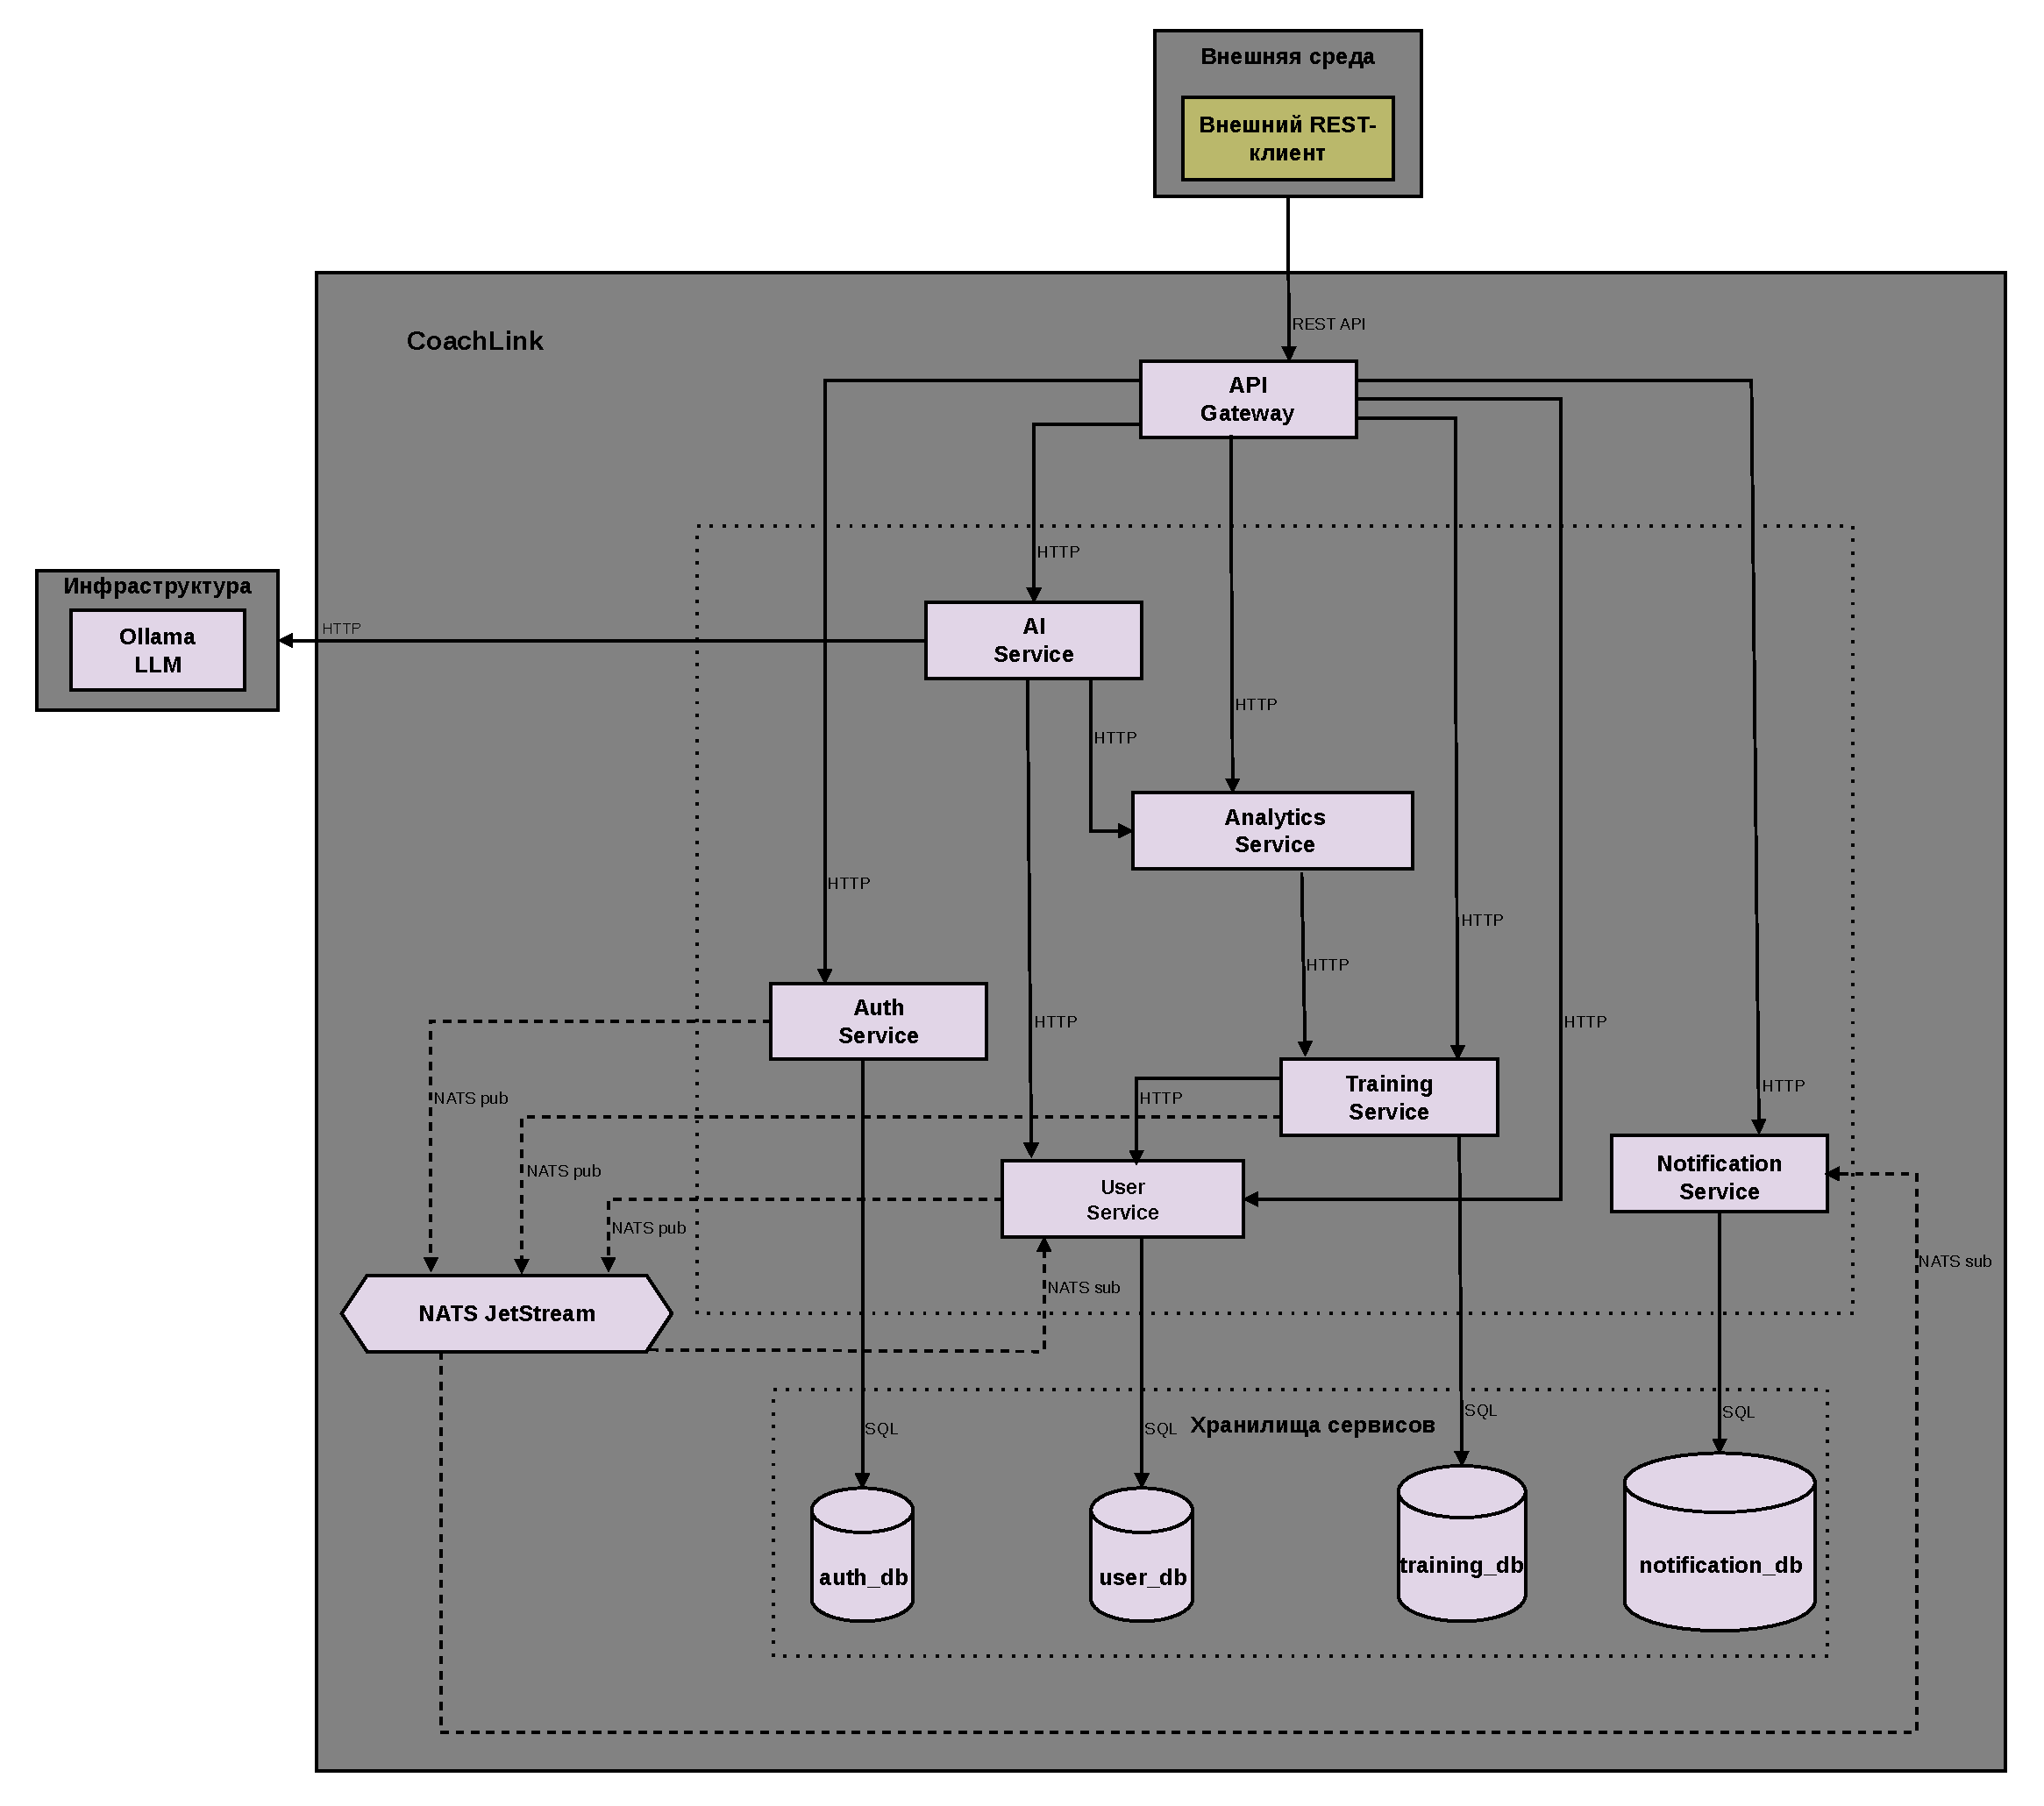
\includegraphics[page=1,width=\textwidth]{inc/components-sheme_cropped.pdf}
  \caption{Компонентная схема backend-платформы}
  \label{fig:components-scheme}
\end{figure}

В такой архитектуре API Gateway не содержит бизнес-логики. Его задача --- принять запрос, проверить JWT, добавить служебные заголовки и передать запрос в нужный сервис. Предметные правила остаются внутри соответствующих сервисов.

\subsection{Состав сервисов}

\subsubsection{API Gateway}

API Gateway является входной точкой для всех публичных HTTP-запросов. Он решает следующие задачи:

\begin{itemize}
\tightlist
\item
  маршрутизация запросов по префиксам;
\item
  проверка JWT access token;
\item
  извлечение идентификатора пользователя, роли и логина из токена;
\item
  проброс пользовательского контекста во внутренние сервисы через заголовки;
\item
  обработка CORS;
\item
  предоставление health-check endpoint.
\end{itemize}

Публичные маршруты без авторизации ограничены регистрацией, входом и обновлением токена:

\begin{itemize}
\tightlist
\item
  \passthrough{\lstinline!POST /api/v1/auth/register!};
\item
  \passthrough{\lstinline!POST /api/v1/auth/login!};
\item
  \passthrough{\lstinline!POST /api/v1/auth/refresh!}.
\end{itemize}

Остальные маршруты требуют заголовок \passthrough{\lstinline!Authorization: Bearer <token>!}. После успешной проверки Gateway устанавливает заголовки:

\begin{itemize}
\tightlist
\item
  \passthrough{\lstinline!X-User-ID!};
\item
  \passthrough{\lstinline!X-User-Role!};
\item
  \passthrough{\lstinline!X-User-Login!}.
\end{itemize}

Такой подход реализует паттерн API Gateway, описанный в работах по микросервисной архитектуре~\cite{richardson-microservices}: аутентификация выполняется один раз на входе, а внутренние сервисы доверяют Gateway и используют переданные заголовки для авторизации. Это исключает необходимость передавать JWT-секрет каждому сервису и упрощает добавление новых сервисов в систему.

\subsubsection{Auth Service}

Auth Service отвечает за учётные данные и токены. В его область ответственности входят:

\begin{itemize}
\tightlist
\item
  регистрация пользователя;
\item
  валидация логина, email, пароля и роли;
\item
  хеширование пароля;
\item
  вход пользователя;
\item
  выпуск access token и refresh token;
\item
  обновление пары токенов;
\item
  отзыв refresh token при logout;
\item
  публикация события регистрации.
\end{itemize}

Access token реализован как JWT. В payload токена включаются:

\begin{lstlisting}
{
  "sub": "uuid пользователя",
  "login": "user_login",
  "role": "coach | athlete",
  "exp": 1234567890,
  "iat": 1234567890
}
\end{lstlisting}

Refresh token хранится в базе данных не в открытом виде, а в виде SHA-256 хеша. Это снижает риск компрометации токена при утечке базы данных. При refresh старый токен удаляется, а пользователю выдаётся новая пара токенов.

После успешной регистрации Auth Service публикует событие \passthrough{\lstinline!coachlink.user.registered!}. Это событие используется User Service для создания пользовательского профиля.

\subsubsection{User Service}

User Service отвечает за доменную информацию о пользователях. Он не хранит пароли и не выпускает токены. Его задачи:

\begin{itemize}
\tightlist
\item
  хранение профилей пользователей;
\item
  синхронизация профилей из события регистрации;
\item
  поиск пользователей по ФИО и логину;
\item
  управление заявками спортсмена тренеру;
\item
  управление связями тренер-спортсмен;
\item
  управление тренировочными группами;
\item
  предоставление внутренних API для других сервисов.
\end{itemize}

Связь тренера и спортсмена создаётся через заявку. Это решение выбрано для явного контроля доступа: спортсмен не может автоматически прикрепиться к тренеру без подтверждения. Тренер видит входящие заявки и может принять или отклонить их.

Тренировочные группы принадлежат тренеру. Добавлять в группу можно только спортсменов, которые уже связаны с этим тренером. Это предотвращает ситуацию, когда тренер назначает тренировку спортсмену, не входящему в его область ответственности.

\subsubsection{Training Service}

Training Service реализует центральную предметную логику платформы. Он отвечает за:

\begin{itemize}
\tightlist
\item
  создание тренировочных планов;
\item
  назначение планов спортсменам;
\item
  назначение планов группе;
\item
  получение списка назначений;
\item
  фильтрацию назначений;
\item
  удаление и архивирование назначений;
\item
  отправку отчётов;
\item
  хранение шаблонов тренировок;
\item
  предоставление внутренних API для аналитики.
\end{itemize}

Тренировочный план и назначение спроектированы как отдельные сущности, связанные отношением <<один ко многим>>. План содержит название, описание и дату тренировки, а назначение связывает план с конкретным спортсменом и хранит индивидуальный статус выполнения. Такое разделение необходимо для групповых тренировок: тренер создаёт один план, а система формирует отдельное назначение для каждого участника группы. Денормализация ФИО и логина спортсмена в таблице назначений позволяет фильтровать и отображать списки без дополнительных запросов в User Service, что устраняет проблему N+1 запросов при получении списка назначений тренера.

Назначение имеет статус:

\begin{itemize}
\tightlist
\item
  \passthrough{\lstinline!assigned!} --- задание назначено и ожидает отчёта;
\item
  \passthrough{\lstinline!completed!} --- спортсмен отправил отчёт;
\item
  \passthrough{\lstinline!archived!} --- тренер перенёс выполненное задание в архив.
\end{itemize}

Просроченность не хранится как отдельное поле, а вычисляется при чтении. Это уменьшает риск рассинхронизации данных. Назначение считается просроченным, если оно находится в статусе \passthrough{\lstinline!assigned!}, а дата выполнения уже прошла.

\subsubsection{Notification Service}

Notification Service реализует паттерн событийного подписчика: он не вызывается напрямую другими сервисами, а подписывается на события NATS JetStream и реагирует на них созданием записей в таблице \passthrough{\lstinline!notifications!}. Для каждого типа события создаётся отдельный durable consumer, что обеспечивает независимую обработку и позволяет восстановить пропущенные сообщения после перезапуска сервиса.

Сервис обрабатывает следующие события:

\begin{itemize}
\tightlist
\item
  заявка спортсмена тренеру;
\item
  принятие или отклонение заявки;
\item
  назначение тренировки;
\item
  удаление задания;
\item
  отправка отчёта;
\item
  добавление спортсмена в группу;
\item
  удаление спортсмена из группы.
\end{itemize}

Пользователь может получить список уведомлений, отфильтровать их по признаку прочтения, получить количество непрочитанных уведомлений в ответе списка и отметить уведомления как прочитанные. Также сервис хранит FCM-токены устройств. Если Firebase credentials не настроены, push-доставка отключается, но уведомления продолжают сохраняться в базе данных.

\subsubsection{Analytics Service}

Analytics Service является stateless-сервисом. Он не имеет собственной базы данных, а получает данные из Training Service через внутренние API. Такое решение исключает проблему синхронизации аналитической базы с основной базой тренировок и гарантирует, что результаты агрегации всегда вычисляются по актуальным данным. При необходимости масштабирования аналитика может быть вынесена в отдельное хранилище без изменения публичного API.

Сервис предоставляет три основных представления данных:

\begin{itemize}
\tightlist
\item
  сводку по спортсмену;
\item
  прогресс по неделям или месяцам;
\item
  обзор по спортсменам тренера.
\end{itemize}

Каждое представление формируется из набора ключевых метрик тренировочного процесса:

\begin{itemize}
\tightlist
\item
  количество отчётов;
\item
  суммарная длительность;
\item
  средняя длительность;
\item
  суммарная дистанция;
\item
  средняя воспринимаемая нагрузка;
\item
  средний пульс;
\item
  максимальный пульс;
\item
  количество назначений;
\item
  процент выполнения.
\end{itemize}

\subsubsection{AI Service}

AI Service отвечает за генерацию рекомендаций по тренировочному процессу конкретного спортсмена на основе накопленных данных.

Публичный endpoint:

\begin{lstlisting}
POST /api/v1/ai/athletes/{id}/recommendations
\end{lstlisting}

Сервис доступен только тренеру. Перед генерацией он проверяет через User Service, что спортсмен действительно связан с текущим тренером. Затем AI Service получает из Analytics Service сводную статистику и последние отчёты спортсмена. Количество отчётов ограничено пятью, чтобы prompt оставался компактным. Типовой сценарий --- рекомендации по последним 3-5 тренировкам.

Генерация выполняется через Ollama. Prompt составляется на русском языке и содержит конкретные данные: объём тренировок, длительность, дистанцию, субъективную нагрузку, пульс и комментарии спортсмена. AI-модуль является вспомогательным инструментом и не заменяет решение тренера.

\subsection{Модель данных}

\subsubsection{Auth Service}

Auth Service использует две основные таблицы (таблица~\ref{tab:auth-db-tables}).

\begin{longtable}[]{|
  >{\raggedright\arraybackslash}p{(\columnwidth - 5\tabcolsep) * \real{0.4700}}|
  >{\raggedright\arraybackslash}p{(\columnwidth - 2\tabcolsep) * \real{0.4700}}|}
\caption{Таблицы Auth Service и их назначение}\label{tab:auth-db-tables}\\
\hline
\begin{minipage}[b]{\linewidth}\raggedright
Таблица
\end{minipage} & \begin{minipage}[b]{\linewidth}\raggedright
Назначение
\end{minipage} \\
\hline
\endhead
\hline
\endlastfoot
\passthrough{\lstinline!users!} & Учётные данные пользователя, роль и пароль в виде bcrypt-хеша \\ \hline
\passthrough{\lstinline!refresh\_tokens!} & Хеши refresh-токенов и срок их действия \\ \hline
\end{longtable}

Таблица \passthrough{\lstinline!users!} содержит логин, email, ФИО, роль, хеш пароля и временные метки. Роль ограничена значениями \passthrough{\lstinline!coach!} и \passthrough{\lstinline!athlete!} через CHECK-констрейнт, что исключает появление невалидных ролей на уровне базы данных. Логин имеет ограничение уникальности. Таблица \passthrough{\lstinline!refresh\_tokens!} связана с пользователем через внешний ключ с каскадным удалением: при удалении пользователя все его refresh-токены удаляются автоматически.

\subsubsection{User Service}

User Service использует следующие таблицы (таблица~\ref{tab:user-db-tables}).

\begin{longtable}[]{|
  >{\raggedright\arraybackslash}p{(\columnwidth - 2\tabcolsep) * \real{0.4700}}|
  >{\raggedright\arraybackslash}p{(\columnwidth - 2\tabcolsep) * \real{0.4700}}|}
\caption{Таблицы User Service и их назначение}\label{tab:user-db-tables}\\
\hline
\begin{minipage}[b]{\linewidth}\raggedright
Таблица
\end{minipage} & \begin{minipage}[b]{\linewidth}\raggedright
Назначение
\end{minipage} \\
\hline
\endhead
\hline
\endlastfoot
\passthrough{\lstinline!user\_profiles!} & Профили пользователей, синхронизированные из Auth Service \\ \hline
\passthrough{\lstinline!connection\_requests!} & Заявки спортсмена тренеру \\ \hline
\passthrough{\lstinline!coach\_athlete\_relations!} & Активные связи тренер-спортсмен \\ \hline
\passthrough{\lstinline!training\_groups!} & Тренировочные группы тренера \\ \hline
\passthrough{\lstinline!training\_group\_members!} & Состав тренировочных групп \\ \hline
\end{longtable}

Разделение \passthrough{\lstinline!users!} и \passthrough{\lstinline!user\_profiles!} отражает разделение ответственности сервисов: Auth Service хранит учётные данные, User Service --- доменную информацию для поиска, связей и групп. Таблица \passthrough{\lstinline!coach\_athlete\_relations!} использует UNIQUE-констрейнт на \passthrough{\lstinline!athlete\_id!}, что ограничивает спортсмена одним тренером и упрощает логику авторизации в Training Service и Analytics Service. Для текстового поиска по ФИО и логину используются trigram-индексы расширения \passthrough{\lstinline!pg\_trgm!}, обеспечивающие поиск подстрок и автодополнение.

\subsubsection{Training Service}

Training Service использует таблицы, описанные в таблице~\ref{tab:training-db-tables}.

\begin{longtable}{|>{\raggedright\arraybackslash}p{0.42\columnwidth}|>{\raggedright\arraybackslash}p{0.46\columnwidth}|}
\caption{Таблицы Training Service и их назначение}\label{tab:training-db-tables}\\
\hline
Таблица & Назначение \\
\hline
\endhead
\hline
\endlastfoot
\passthrough{\lstinline!training\_plans!} & Общая информация о тренировочном плане \\ \hline
\passthrough{\lstinline!training\_assignments!} & Назначение плана конкретному спортсмену \\ \hline
\passthrough{\lstinline!training\_reports!} & Отчёт спортсмена по назначению \\ \hline
\passthrough{\lstinline!training\_templates!} & Шаблоны тренировок тренера \\ \hline
\end{longtable}

Разделение плана и назначения на уровне таблиц соответствует проектному решению, описанному в разделе 2.3: один план порождает несколько назначений при групповой тренировке. Таблица \passthrough{\lstinline!training\_assignments!} содержит внешний ключ на план с каскадным удалением, CHECK-констрейнт на статус и денормализованные поля ФИО спортсмена. Отчёт связан с назначением через UNIQUE-ограничение: каждому назначению соответствует не более одного отчёта. Поле \passthrough{\lstinline!perceived\_effort!} ограничено диапазоном от 0 до 10 через CHECK-констрейнт.

\subsubsection{Notification Service}

Notification Service хранит данные в таблицах, представленных в таблице~\ref{tab:notification-db-tables}.

\begin{longtable}{|>{\raggedright\arraybackslash}p{0.42\columnwidth}|>{\raggedright\arraybackslash}p{0.46\columnwidth}|}
\caption{Таблицы Notification Service и их назначение}\label{tab:notification-db-tables}\\
\hline
Таблица & Назначение \\
\hline
\endhead
\hline
\endlastfoot
\passthrough{\lstinline!notifications!} & Уведомления пользователей \\ \hline
\passthrough{\lstinline!device\_tokens!} & FCM-токены устройств \\ \hline
\end{longtable}

В уведомлении хранится тип, заголовок, текст, дополнительные данные в JSONB, признак прочтения и дата создания. JSONB-поле позволяет добавлять к уведомлению контекст: идентификатор заявки, задания или группы.

\subsubsection{ER-диаграмма}

Общая структура данных представлена на ER-диаграмме (рисунок~\ref{fig:er-diagram}). Диаграмма отражает логические связи между основными сущностями платформы. В микросервисной архитектуре таблицы физически распределены по базам данных отдельных сервисов.

\begin{figure}[H]
  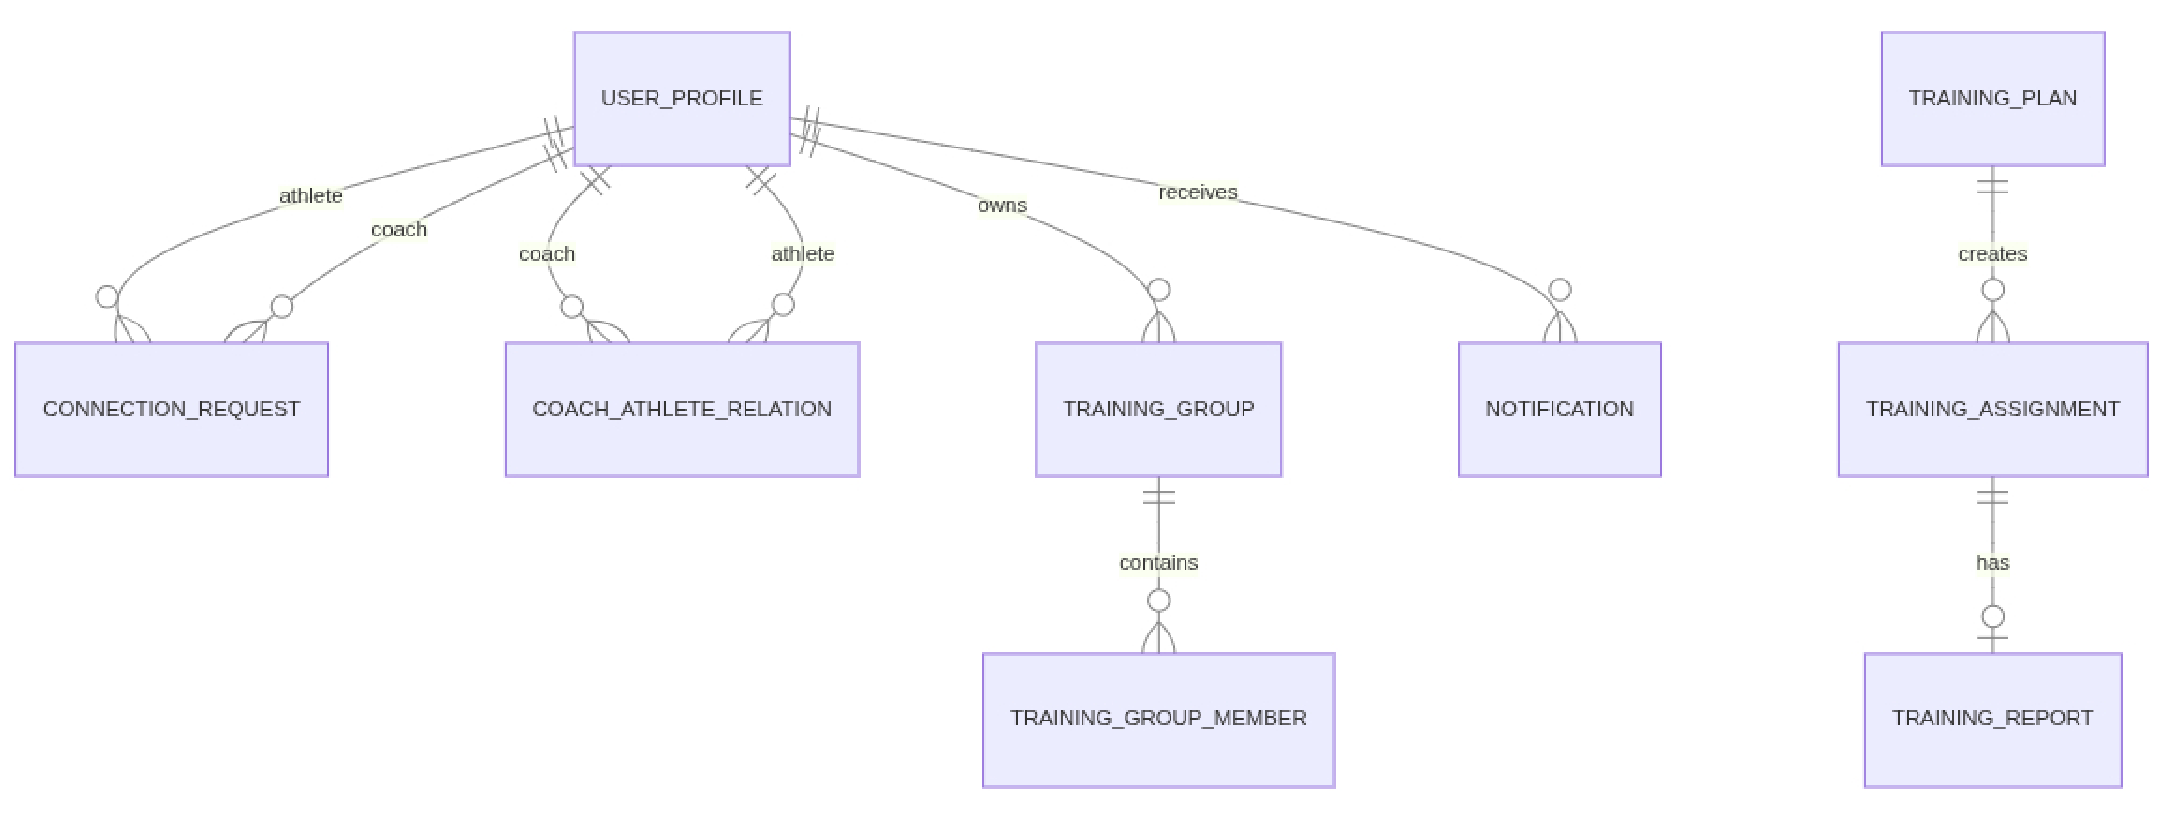
\includegraphics[page=1,width=\textwidth]{inc/ER-diagram_cropped.pdf}
  \caption{ER-диаграмма основных сущностей платформы CoachLink}
  \label{fig:er-diagram}
\end{figure}

\subsection{Межсервисное взаимодействие}

\subsubsection{Синхронное взаимодействие}

Синхронные HTTP-вызовы используются в случаях, когда результат нужен для выполнения текущего запроса.

Примеры:

\begin{enumerate}
\def\labelenumi{\arabic{enumi}.}
\tightlist
\item
  Training Service обращается к User Service при назначении плана группе, чтобы получить список участников группы;
\item
  Training Service получает профиль спортсмена, чтобы сохранить имя и логин в назначении;
\item
  Analytics Service обращается к Training Service за отчётами и агрегатами;
\item
  AI Service обращается к User Service для проверки связи тренера и спортсмена;
\item
  AI Service обращается к Analytics Service за сводкой и последними отчётами.
\end{enumerate}

Внутренние API не предназначены для внешних клиентов и доступны только сервисам внутри backend-платформы. При недоступности вызываемого сервиса вызывающий сервис возвращает клиенту ошибку с соответствующим HTTP-статусом. Повторные попытки для синхронных запросов не применяются, поскольку клиент ожидает ответ и повтор увеличил бы время ожидания. Для операций, допускающих задержку, используется асинхронное взаимодействие через NATS JetStream, где гарантия доставки обеспечивается брокером сообщений.

\subsubsection{Асинхронное взаимодействие}

Асинхронное взаимодействие реализовано через NATS JetStream. Оно используется там, где действие может быть выполнено после основного запроса и не должно блокировать пользователя.

Например, при создании тренировочного назначения Training Service публикует событие \passthrough{\lstinline!coachlink.training.assigned!}. Notification Service получает событие и создаёт уведомление для спортсмена. Если Notification Service временно недоступен, JetStream durable consumer позволяет обработать событие после восстановления сервиса.

В таблице~\ref{tab:nats-key-events} приведён список ключевых событий.

\begin{longtable}{|
  >{\raggedright\arraybackslash}p{0.34\columnwidth}|
  >{\raggedright\arraybackslash}p{0.16\columnwidth}|
  >{\raggedright\arraybackslash}p{0.18\columnwidth}|
  >{\raggedright\arraybackslash}p{0.20\columnwidth}|}
\caption{Ключевые события NATS JetStream в backend-платформе}\label{tab:nats-key-events}\\
\hline
Событие & Источник & Получатель & Назначение \\
\hline
\endfirsthead
\caption[]{Продолжение таблицы \thetable}\\
\hline
Событие & Источник & Получатель & Назначение \\
\hline
\endhead
\hline
\endlastfoot
\path|coachlink.user.registered| & Auth Service & User Service & Создание профиля \\ \hline
\path|coachlink.connection.requested| & User Service & Notification Service & Уведомление тренера \\ \hline
\path|coachlink.connection.accepted| & User Service & Notification Service & Уведомление спортсмена \\ \hline
\path|coachlink.connection.rejected| & User Service & Notification Service & Уведомление спортсмена \\ \hline
\path|coachlink.group.athlete_added| & User Service & Notification Service & Уведомление спортсмена \\ \hline
\path|coachlink.group.athlete_removed| & User Service & Notification Service & Уведомление спортсмена \\ \hline
\path|coachlink.training.assigned| & Training Service & Notification Service & Уведомление спортсмена \\ \hline
\path|coachlink.training.deleted| & Training Service & Notification Service & Уведомление спортсмена \\ \hline
\path|coachlink.report.submitted| & Training Service & Notification Service & Уведомление тренера \\ \hline
\end{longtable}

\subsection{Проектирование ключевых сценариев}

\subsubsection{Регистрация пользователя}

Сценарий регистрации включает несколько шагов: клиент отправляет запрос через API Gateway, Auth Service валидирует данные, хеширует пароль, создаёт пользователя и публикует событие в NATS JetStream, после чего User Service создаёт профиль. На рисунке~\ref{fig:registration-flow} показана последовательность взаимодействий при регистрации.

\begin{figure}[H]
  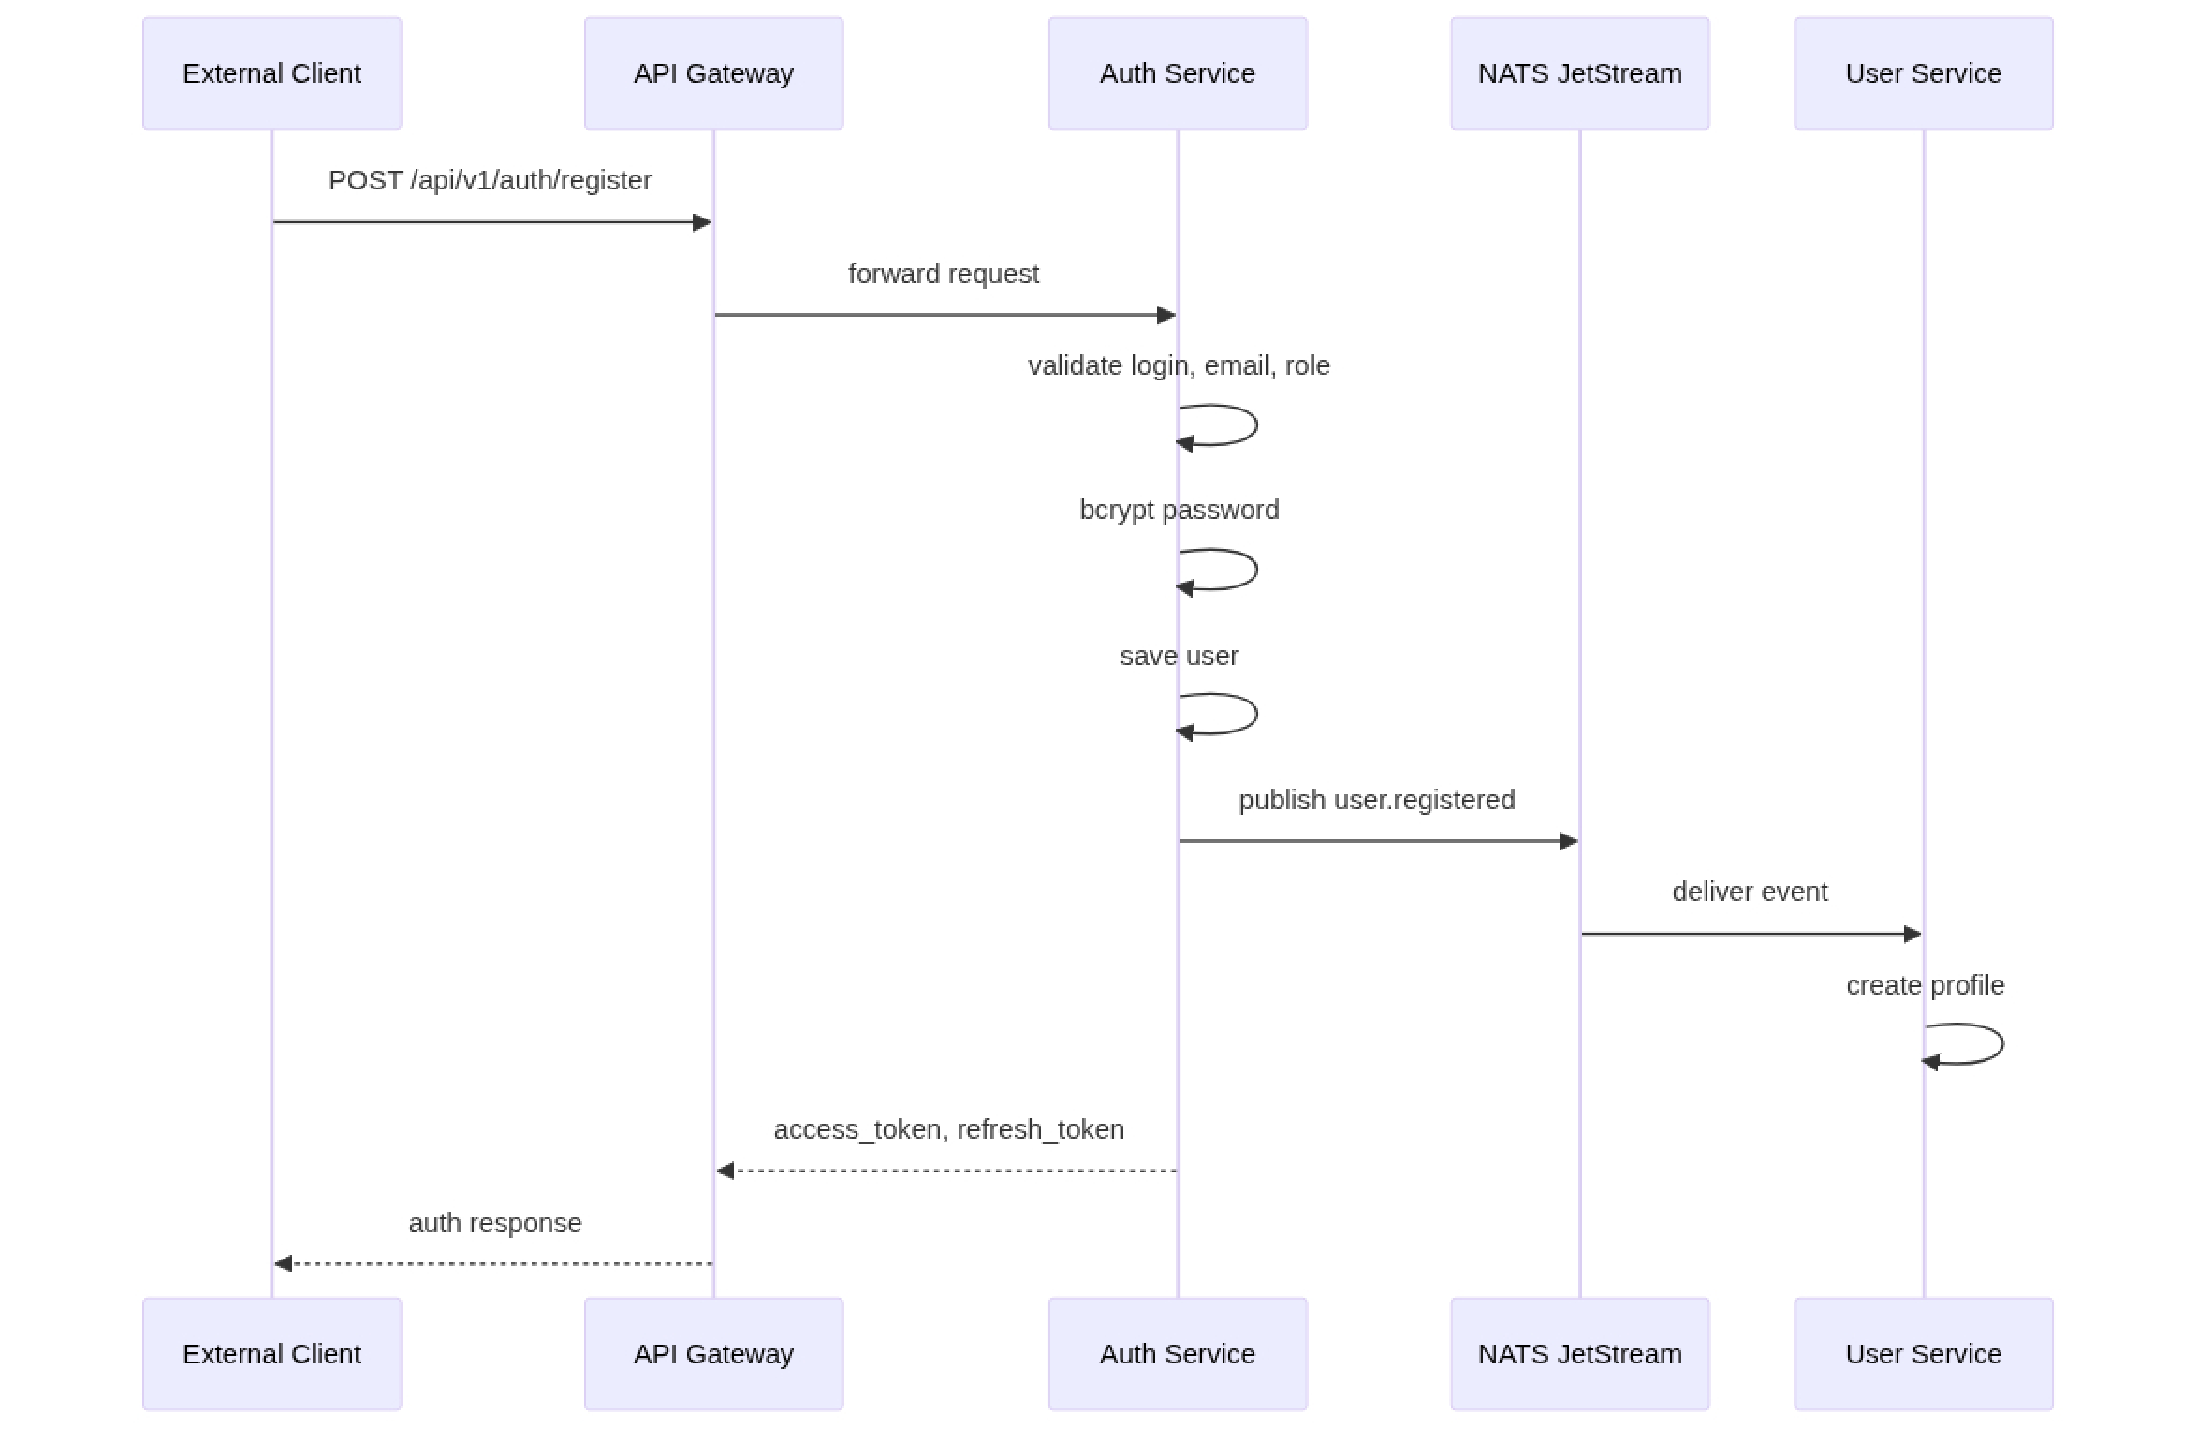
\includegraphics[page=1,width=\textwidth]{inc/user-registration_cropped.pdf}
  \caption{Последовательность взаимодействий при регистрации пользователя}
  \label{fig:registration-flow}
\end{figure}

\subsubsection{Создание связи тренер-спортсмен}

Для установления связи спортсмен отправляет заявку тренеру. Тренер получает уведомление и принимает или отклоняет заявку. При принятии создаётся запись в таблице связей. На рисунке~\ref{fig:coach-athlete-flow} представлена последовательность взаимодействий при создании связи.

\begin{figure}[H]
  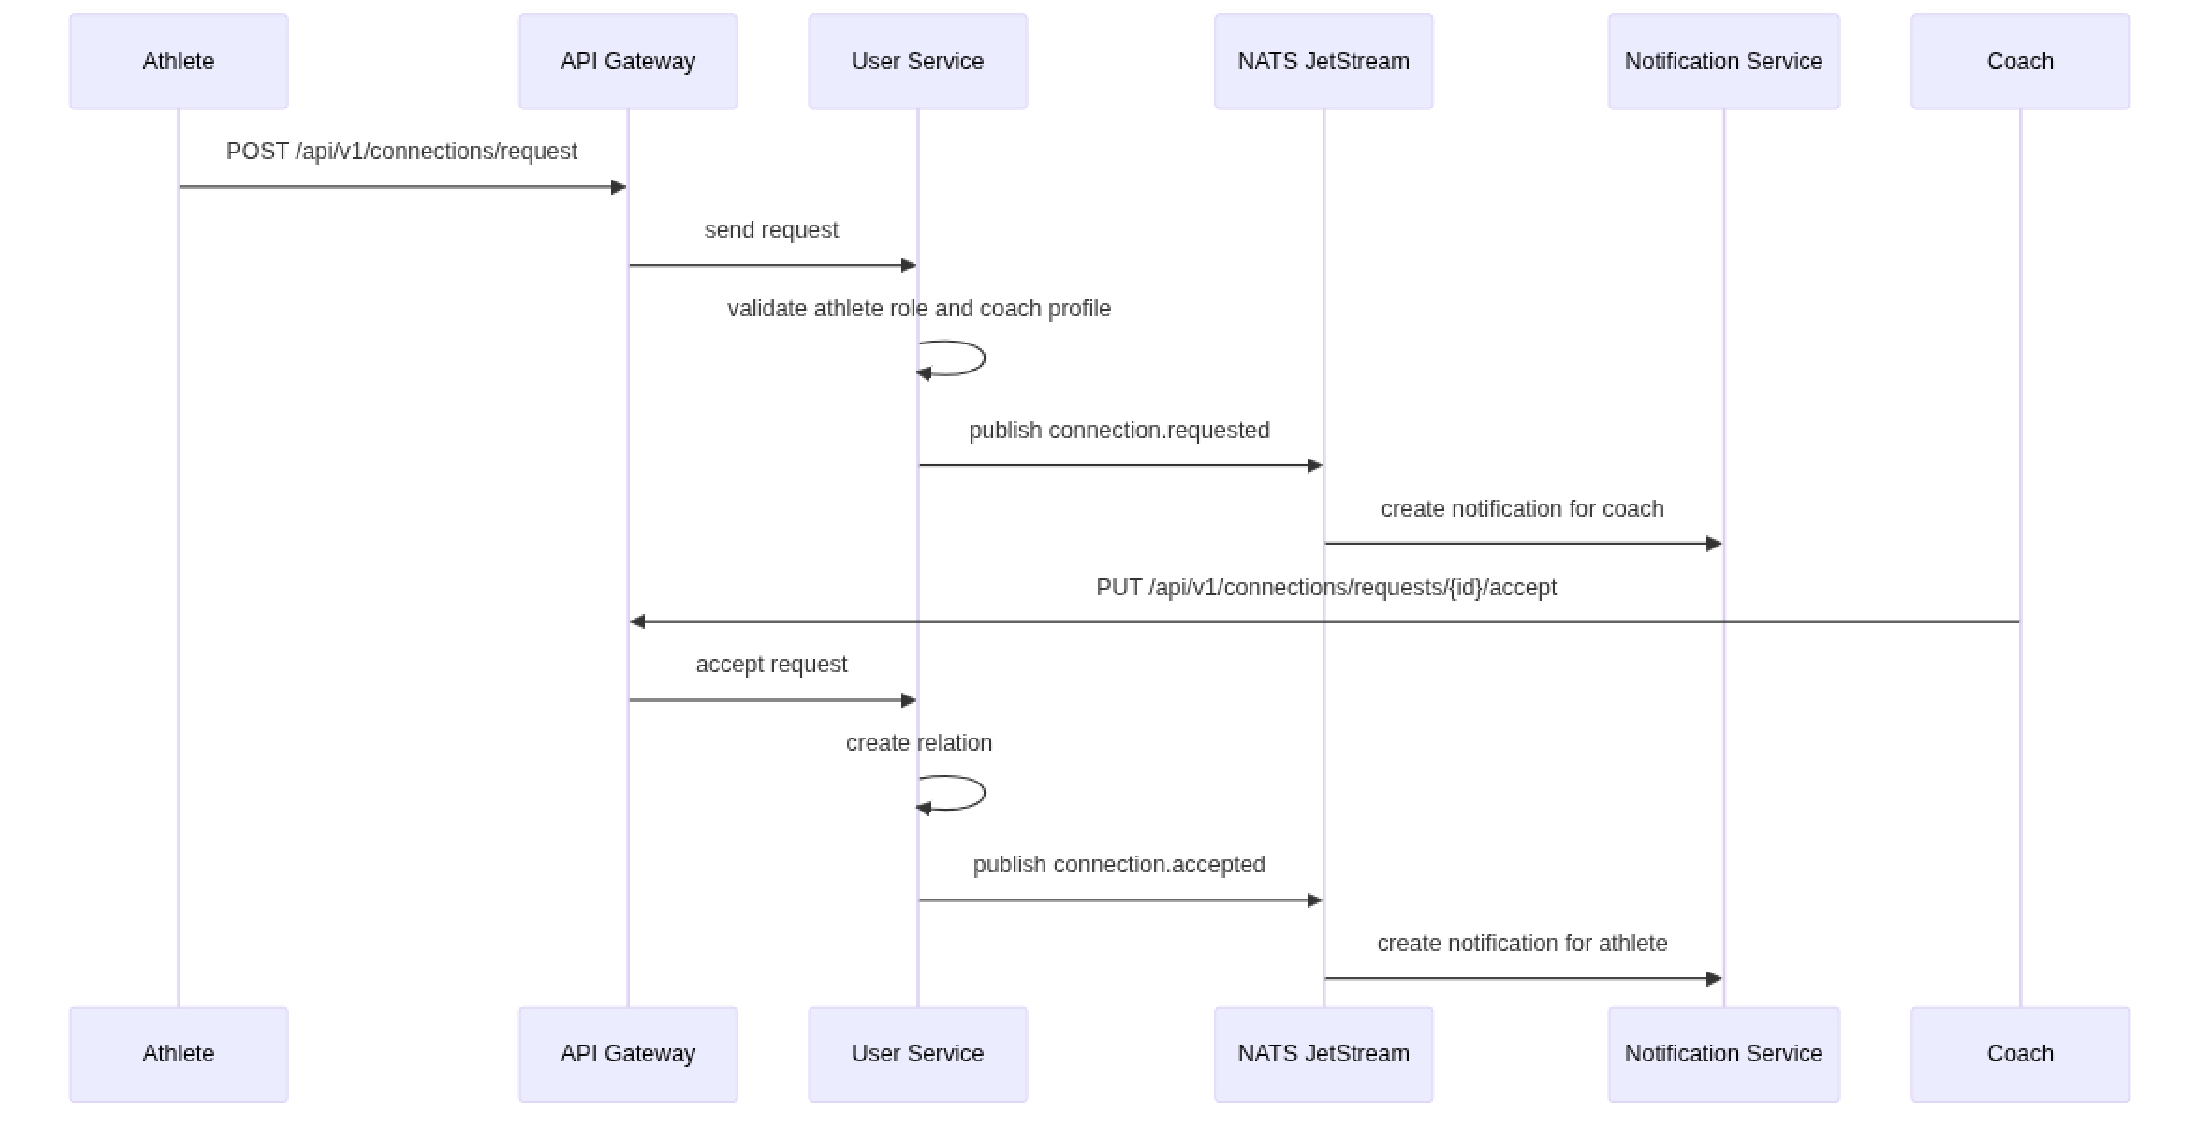
\includegraphics[page=1,width=\textwidth]{inc/user-coach_cropped.pdf}
  \caption{Последовательность взаимодействий при создании связи тренер-спортсмен}
  \label{fig:coach-athlete-flow}
\end{figure}

\subsubsection{Назначение тренировки группе}

При назначении тренировки группе Training Service обращается к User Service для получения списка участников, затем создаёт отдельное назначение для каждого спортсмена и публикует событие для Notification Service. На рисунке~\ref{fig:group-assignment-flow} показана последовательность взаимодействий при назначении тренировки группе.

\begin{figure}[H]
  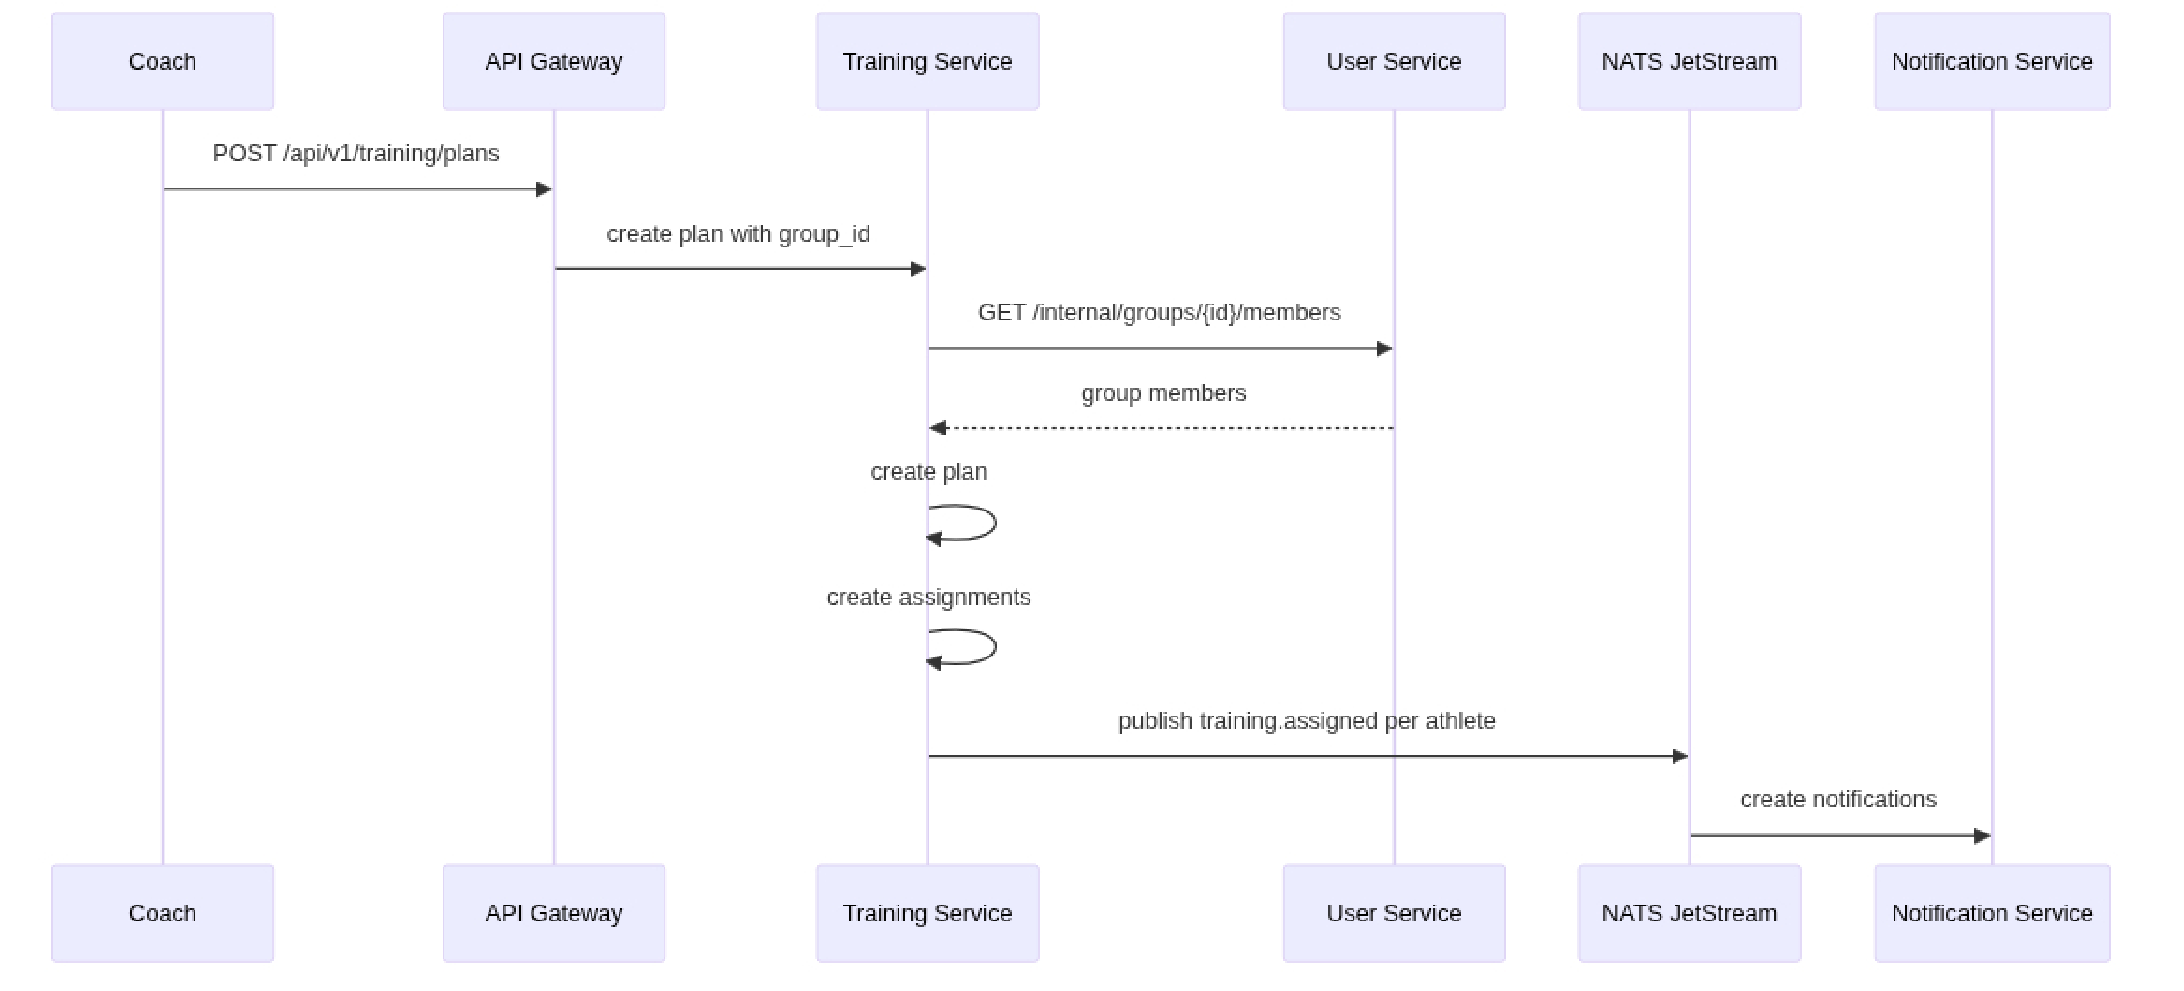
\includegraphics[page=1,width=\textwidth]{inc/trenirovka-grupe_cropped.pdf}
  \caption{Последовательность взаимодействий при назначении тренировки группе}
  \label{fig:group-assignment-flow}
\end{figure}

\subsubsection{Отправка отчёта}

При отправке отчёта спортсмен передаёт данные через API Gateway в Training Service. Сервис проверяет принадлежность назначения, сохраняет отчёт, меняет статус назначения и публикует событие, на которое реагирует Notification Service. На рисунке~\ref{fig:report-flow} показана последовательность взаимодействий при отправке отчёта.

\begin{figure}[H]
  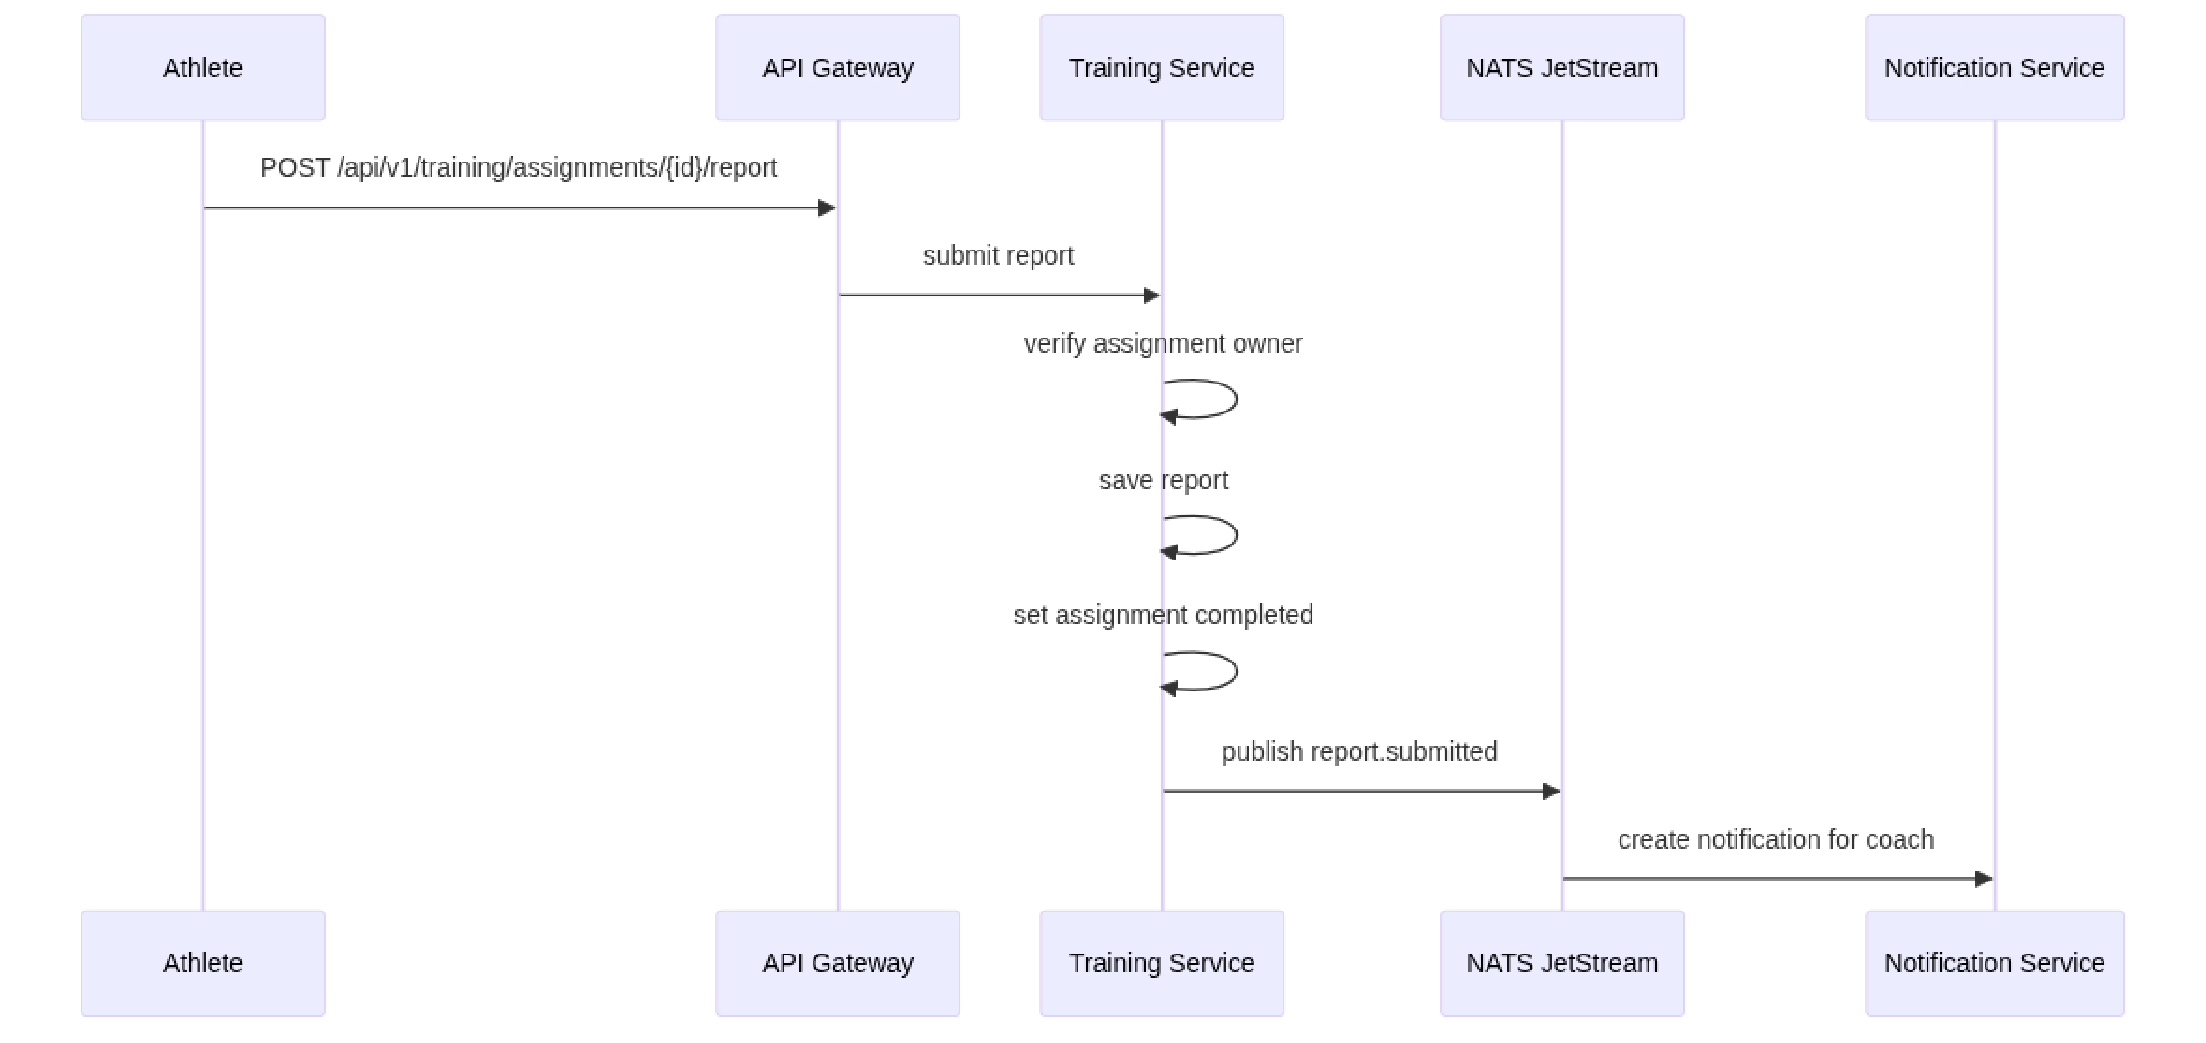
\includegraphics[page=1,width=\textwidth]{inc/report-sending_cropped.pdf}
  \caption{Последовательность взаимодействий при отправке отчёта}
  \label{fig:report-flow}
\end{figure}

\subsubsection{Получение AI-рекомендации}

Для получения AI-рекомендации тренер отправляет запрос через API Gateway в AI Service. Сервис проверяет связь тренера и спортсмена через User Service, получает статистику и последние отчёты из Analytics Service, формирует prompt и обращается к Ollama для генерации текста. На рисунке~\ref{fig:ai-recommendation-flow} показана последовательность взаимодействий при получении AI-рекомендации.

\begin{figure}[H]
  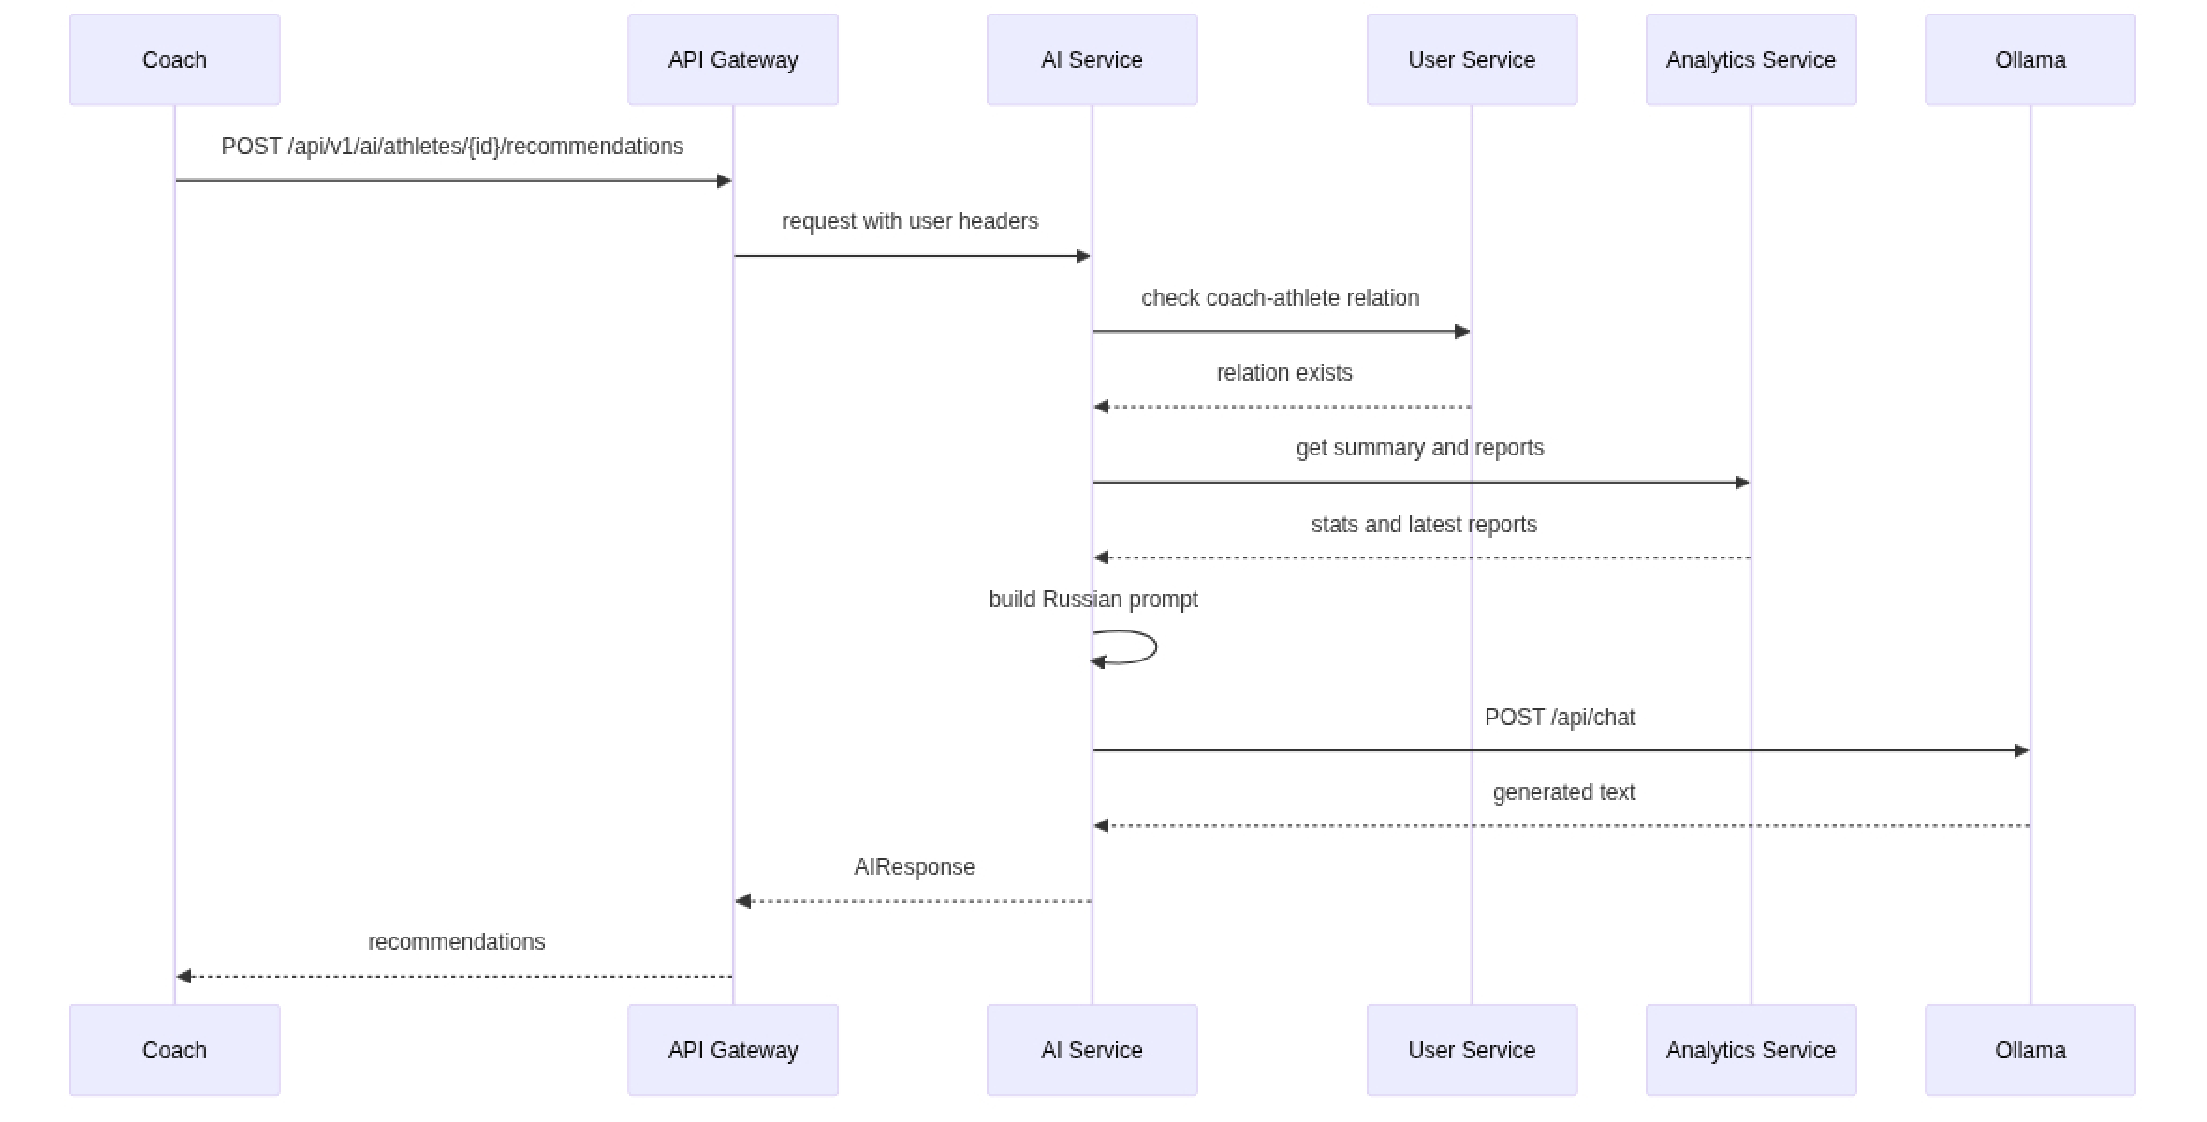
\includegraphics[page=1,width=\textwidth]{inc/AI-recomendation_cropped.pdf}
  \caption{Последовательность взаимодействий при получении AI-рекомендации}
  \label{fig:ai-recommendation-flow}
\end{figure}

\subsection{Проектирование публичного API}

Публичный API разделён на группы по предметным областям (таблица~\ref{tab:public-api-groups}).

\begin{longtable}{|>{\raggedright\arraybackslash}p{0.42\columnwidth}|>{\raggedright\arraybackslash}p{0.46\columnwidth}|}
\caption{Группы публичного API CoachLink}\label{tab:public-api-groups}\\
\hline
Группа & Назначение \\
\hline
\endfirsthead
\caption[]{Продолжение таблицы \thetable}\\
\hline
Группа & Назначение \\
\hline
\endhead
\hline
\endlastfoot
\passthrough{\lstinline!/api/v1/auth/*!} & Регистрация, вход, обновление и отзыв токенов \\ \hline
\passthrough{\lstinline!/api/v1/users/*!} & Профиль текущего пользователя и поиск \\ \hline
\passthrough{\lstinline!/api/v1/connections/*!} & Заявки и связи тренер-спортсмен \\ \hline
\passthrough{\lstinline!/api/v1/groups/*!} & Тренировочные группы \\ \hline
\passthrough{\lstinline!/api/v1/training/*!} & Планы, назначения, отчёты, шаблоны \\ \hline
\passthrough{\lstinline!/api/v1/notifications/*!} & Уведомления \\ \hline
\passthrough{\lstinline!/api/v1/analytics/*!} & Аналитика тренировок \\ \hline
\passthrough{\lstinline!/api/v1/ai/*!} & AI-рекомендации \\ \hline
\end{longtable}

Такое разделение упрощает маршрутизацию на уровне API Gateway и позволяет документировать каждую группу endpoint-ов независимо. При проектировании API соблюдались следующие принципы: версионирование через префикс \passthrough{\lstinline!/v1/!}, что позволяет вводить несовместимые изменения в будущих версиях без нарушения работы существующих клиентов; единообразный формат ошибок с HTTP-статусом и JSON-телом, содержащим описание ошибки; пагинация списков через query-параметры \passthrough{\lstinline!limit!} и \passthrough{\lstinline!offset!}; использование стандартных HTTP-методов в соответствии с семантикой REST. Полная спецификация API оформлена в формате OpenAPI и доступна в репозитории проекта.

\subsection{Расширяемость под другие виды спорта}

Хотя первая версия ориентирована на лёгкую атлетику, архитектура спроектирована с учётом расширения на другие виды спорта. Базовые сущности платформы --- пользователи, роли, связи, группы, назначения, уведомления и аналитические агрегаты --- не зависят от конкретного вида спорта и остаются неизменными при добавлении новых дисциплин.

Расширение предметной модели сосредоточено в Training Service. Конкретный механизм состоит в добавлении sport-specific полей в структуру тренировочного плана и отчёта. Например, для силовых видов спорта потребуются параметры подходов, повторений и веса, для плавания --- стиль и длина бассейна, для велоспорта --- средняя мощность и набор высоты. Эти поля могут быть реализованы через расширение схемы таблиц или через JSONB-поле с динамической структурой. При этом общий жизненный цикл назначения (создание, выполнение, отчёт, архивация), система уведомлений, аналитическая агрегация и API Gateway не требуют изменений.

\subsection{Выводы по главе 2}

В проектной части была предложена микросервисная backend-архитектура CoachLink. Архитектура включает API Gateway, сервис авторизации, сервис пользователей, сервис тренировок, сервис уведомлений, сервис аналитики и AI-сервис рекомендаций. Для хранения данных используется PostgreSQL, для событийного взаимодействия --- NATS JetStream, для локального развёртывания --- Docker Compose.

Спроектированная архитектура соответствует требованиям, сформулированным в аналитической главе. Она поддерживает ролевую модель, связи тренера и спортсмена, групповые назначения, стандартизированные отчёты, уведомления и аналитику. При этом система остаётся расширяемой: текущая реализация ориентирована на лёгкую атлетику, но базовая модель может быть адаптирована для других видов спорта.

    \section{РЕАЛИЗАЦИЯ И ТЕСТИРОВАНИЕ}

\subsection{Общая структура реализации}

Backend-платформа CoachLink реализована как набор Go-сервисов в монорепозитории. Выбор монорепозитория обусловлен упрощением управления общими зависимостями, единой системой сборки и упрощённой координацией изменений между сервисами на этапе активной разработки.

Каждый сервис реализован как самостоятельный Go-модуль со стандартной внутренней структурой: точка входа, конфигурация, HTTP-обработчики, сервисный слой с бизнес-логикой, модели данных и слой доступа к базе данных или внешним клиентам. Общий код, используемый несколькими сервисами, вынесен в разделяемый пакет --- в частности, типы и названия событий NATS JetStream, что обеспечивает согласованность событийных контрактов между публикующими и подписанными сервисами.

Для локального развёртывания используется Docker Compose: все семь сервисов, PostgreSQL, NATS JetStream и Ollama запускаются как контейнеры. Для каждого сервиса предусмотрен отдельный Dockerfile, обеспечивающий воспроизводимую сборку. Stateful-сервисы применяют SQL-миграции при запуске с помощью библиотеки goose, что гарантирует актуальность схемы базы данных без ручного вмешательства. Конфигурация каждого сервиса задаётся через переменные окружения, что упрощает развёртывание в различных средах. Краткое описание назначения каждого сервиса и его взаимодействий приведено в приложении А.

\subsection{API Gateway}

API Gateway реализован как отдельный Go-сервис на основе фреймворка Echo. Проксирование запросов выполняется через \passthrough{\lstinline!net/http/httputil.ReverseProxy!} из стандартной библиотеки Go. Для каждого backend-сервиса создаётся отдельный экземпляр reverse proxy с пользовательским \passthrough{\lstinline!Director!}, который сохраняет полный путь запроса и подменяет только scheme и host целевого сервиса. При ошибке проксирования пользовательский \passthrough{\lstinline!ErrorHandler!} возвращает клиенту ответ 502 в формате JSON.

Входящие запросы проходят через цепочку middleware в фиксированном порядке: восстановление после паники, генерация идентификатора запроса, обработка CORS, структурированное логирование и проверка JWT. Маршрутизация выполняется по префиксам, как показано в таблице~\ref{tab:gateway-routing}.

\begin{longtable}{|>{\raggedright\arraybackslash}p{0.42\columnwidth}|>{\raggedright\arraybackslash}p{0.46\columnwidth}|}
\caption{Маршрутизация API Gateway по префиксам}\label{tab:gateway-routing}\\
\hline
Префикс & Целевой сервис \\
\hline
\endhead
\hline
\endlastfoot
\passthrough{\lstinline!/api/v1/auth/*!} & Auth Service \\ \hline
\passthrough{\lstinline!/api/v1/users/*!} & User Service \\ \hline
\passthrough{\lstinline!/api/v1/connections/*!} & User Service \\ \hline
\passthrough{\lstinline!/api/v1/groups/*!} & User Service \\ \hline
\passthrough{\lstinline!/api/v1/training/*!} & Training Service \\ \hline
\passthrough{\lstinline!/api/v1/notifications/*!} & Notification Service \\ \hline
\passthrough{\lstinline!/api/v1/analytics/*!} & Analytics Service \\ \hline
\passthrough{\lstinline!/api/v1/ai/*!} & AI Service \\ \hline
\end{longtable}

Gateway выполняет JWT-проверку для всех защищённых маршрутов. Исключениями являются регистрация, вход, обновление токена и health-check. После успешной проверки токена Gateway извлекает из полей токена идентификатор пользователя, роль и логин. Эти значения передаются дальше через заголовки, представленные на рисунке~\ref{src:gateway-headers}.

\begin{figure}
\begin{lstlisting}
X-User-ID: <user_id>
X-User-Role: <coach|athlete>
X-User-Login: <login>
\end{lstlisting}
\caption{Заголовки запроса, передаваемые Gateway внутренним сервисам}
\label{src:gateway-headers}
\end{figure}

Такой механизм позволяет внутренним сервисам принимать решения о доступе без повторной проверки JWT. Например, Training Service проверяет, может ли текущий пользователь создать план, отправить отчёт или получить назначение.

Gateway также отвечает за обработку CORS-заголовков, необходимых для корректной работы web-клиентов, и предоставляет health-check endpoint для проверки доступности сервиса.

\subsection{Auth Service}

Auth Service отвечает за регистрацию, вход и управление токенами. Сервис использует PostgreSQL-базу \passthrough{\lstinline!auth\_db!} и таблицы \passthrough{\lstinline!users!} и \passthrough{\lstinline!refresh\_tokens!}.

\subsubsection{Регистрация}

При регистрации пользователь передаёт логин, email, пароль, ФИО и роль. DTO запроса содержит ограничения:

\begin{itemize}
\tightlist
\item
  логин обязателен, длина от 3 до 50 символов;
\item
  email должен иметь корректный формат;
\item
  пароль обязателен, длина от 8 до 128 символов;
\item
  ФИО обязательно;
\item
  роль должна быть \passthrough{\lstinline!coach!} или \passthrough{\lstinline!athlete!}.
\end{itemize}

Дополнительно сервис проверяет формат логина регулярным выражением (рисунок~\ref{src:login-regex}).

\begin{figure}
\begin{lstlisting}
^[a-zA-Z0-9-]+$
\end{lstlisting}
\caption{Регулярное выражение для проверки формата логина}
\label{src:login-regex}
\end{figure}

Это ограничение исключает пробелы, кириллицу и специальные символы в логине, что упрощает поиск и использование логина в API.

Пароль хешируется через bcrypt с cost-фактором 12, что обеспечивает баланс между безопасностью и временем вычисления хеша. В базе хранится только \passthrough{\lstinline!password\_hash!}, исходный пароль не сохраняется. Значение cost-фактора задаётся через переменную окружения и может быть изменено без модификации кода. После создания пользователя сервис публикует событие \passthrough{\lstinline!coachlink.user.registered!}, содержащее идентификатор пользователя, логин, ФИО, email и роль.

\subsubsection{Вход и токены}

При входе сервис ищет пользователя по логину и сравнивает пароль с bcrypt-хешем. При успешной проверке создаётся пара токенов:

\begin{itemize}
\tightlist
\item
  access token --- JWT, подписанный алгоритмом HMAC-SHA256, со сроком жизни 15 минут;
\item
  refresh token --- случайный UUID со сроком жизни 30 дней.
\end{itemize}

Структура полей access token описана в разделе проектирования (рисунок~\ref{src:design-jwt-payload}).

Refresh token не хранится в открытом виде. Сервис вычисляет SHA-256 хеш токена и сохраняет только хеш. Такой подход снижает риск компрометации при утечке базы данных: даже получив содержимое таблицы, злоумышленник не сможет восстановить исходный токен. При refresh старый хеш удаляется из базы, затем создаётся новая пара access/refresh. При logout refresh token также удаляется, что делает невозможным дальнейшее обновление сессии. Auth Service предоставляет четыре публичных endpoint: регистрацию, вход, обновление токена и выход.

\subsection{User Service}

User Service хранит пользовательские профили, связи тренер-спортсмен и тренировочные группы. Он использует базу \passthrough{\lstinline!user\_db!}.

\subsubsection{Синхронизация профилей}

Профиль пользователя создаётся не напрямую при регистрации, а через событие \passthrough{\lstinline!coachlink.user.registered!}. Auth Service публикует событие после успешной регистрации, а User Service подписан на него через NATS JetStream. При получении события User Service создаёт запись в таблице \passthrough{\lstinline!user\_profiles!}.

Такое разделение позволяет Auth Service отвечать только за учётные данные и токены, а User Service --- за доменную информацию, используемую в тренировочном процессе.

\subsubsection{Поиск пользователей}

Сервис предоставляет поиск по ФИО и логину. Поиск используется, например, когда спортсмен ищет тренера для отправки заявки или тренер ищет спортсмена. Минимальная длина поискового запроса --- два символа. Это ограничение снижает нагрузку на индекс при поиске по коротким строкам.

Для ускорения поиска в базе включено расширение \passthrough{\lstinline!pg\_trgm!}, а для полей имени и логина создаются trigram-индексы. Это подходит для поиска подстрок и автодополнения.

\subsubsection{Заявки и связи}

Связь тренера и спортсмена создаётся через заявку. Основной сценарий:

\begin{enumerate}
\def\labelenumi{\arabic{enumi}.}
\tightlist
\item
  спортсмен находит тренера;
\item
  спортсмен отправляет заявку;
\item
  тренер получает уведомление;
\item
  тренер принимает или отклоняет заявку;
\item
  при принятии создаётся запись в \passthrough{\lstinline!coach\_athlete\_relations!}.
\end{enumerate}

В первой версии у спортсмена может быть один тренер. Это ограничение задаётся уникальностью \passthrough{\lstinline!athlete\_id!} в таблице связей. Такое решение упрощает логику доступа: Training Service и Analytics Service могут однозначно определять, какой тренер отвечает за спортсмена.

\subsubsection{Тренировочные группы}

Тренер может создавать тренировочные группы и добавлять туда своих спортсменов. Группа используется для массового назначения тренировочного плана: при создании плана с указанием \passthrough{\lstinline!group\_id!} Training Service запрашивает состав группы через внутренний API User Service и формирует назначения для каждого участника.

Перед добавлением спортсмена в группу сервис проверяет наличие записи в таблице \passthrough{\lstinline!coach\_athlete\_relations!}. Если связь отсутствует, запрос отклоняется. При удалении группы записи в таблице участников удаляются каскадно. При добавлении или удалении спортсмена из группы публикуются события \passthrough{\lstinline!coachlink.group.athlete\_added!} и \passthrough{\lstinline!coachlink.group.athlete\_removed!}, на которые реагирует Notification Service.

\subsubsection{Внутренние API}

User Service предоставляет внутренние API для других сервисов (таблица~\ref{tab:user-internal-api}).

\begin{longtable}[]{|
  >{\raggedright\arraybackslash}p{(\columnwidth - 2\tabcolsep) * \real{0.4700}}|
  >{\raggedright\arraybackslash}p{(\columnwidth - 2\tabcolsep) * \real{0.4700}}|}
\caption{Внутренние API User Service}\label{tab:user-internal-api}\\
\hline
\begin{minipage}[b]{\linewidth}\raggedright
Endpoint
\end{minipage} & \begin{minipage}[b]{\linewidth}\raggedright
Использование
\end{minipage} \\
\hline
\endfirsthead
\caption*{Продолжение таблицы \ref{tab:user-internal-api}}\\
\hline
\begin{minipage}[b]{\linewidth}\raggedright
Endpoint
\end{minipage} & \begin{minipage}[b]{\linewidth}\raggedright
Использование
\end{minipage} \\
\hline
\endhead
\hline
\endlastfoot
GET \path|/internal/users/{userId}| & Получение профиля пользователя \\ \hline
GET \path|/internal/groups/{groupId}/members| & Получение состава группы \\ \hline
GET \path|/internal/coach/{coachId}/has-athlete/{athleteId}| & Проверка связи тренера и спортсмена \\ \hline
\end{longtable}

Эти API не предназначены для внешних клиентов. Они позволяют Training Service, Analytics Service и AI Service выполнять предметные проверки и получать необходимые данные.

\subsection{Training Service}

Training Service является центральным сервисом тренировочного процесса. Он использует базу \passthrough{\lstinline!training\_db!}.

\subsubsection{Тренировочные планы}

Тренировочный план содержит название, описание, дату и идентификатор тренера. План может быть назначен:

\begin{itemize}
\tightlist
\item
  одному или нескольким спортсменам по списку \passthrough{\lstinline!athlete\_ids!};
\item
  всем спортсменам группы через \passthrough{\lstinline!group\_id!};
\item
  комбинации группы и отдельных спортсменов.
\end{itemize}

Если указан \passthrough{\lstinline!group\_id!}, Training Service обращается к User Service и получает участников группы. Участники группы и спортсмены из \passthrough{\lstinline!athlete\_ids!} объединяются через ассоциативный массив с дедупликацией по идентификатору: если спортсмен указан одновременно в группе и в списке, он получит только одно назначение. Затем создаётся один тренировочный план и набор назначений для каждого спортсмена. При этом используется стратегия частичного успеха: если создание назначения для одного из спортсменов завершается ошибкой, остальные назначения продолжают создаваться.

\subsubsection{Назначения}

Назначение представляет связь между тренировочным планом и конкретным спортсменом. В назначении хранятся:

\begin{itemize}
\tightlist
\item
  \passthrough{\lstinline!plan\_id!};
\item
  \passthrough{\lstinline!athlete\_id!};
\item
  \passthrough{\lstinline!coach\_id!};
\item
  имя и логин спортсмена;
\item
  имя и логин тренера;
\item
  статус;
\item
  время назначения;
\item
  время выполнения;
\item
  время архивации.
\end{itemize}

Денормализация имени и логина спортсмена используется для фильтрации списков назначений без дополнительного запроса в User Service.

Статусы назначений приведены в таблице~\ref{tab:assignment-statuses}.

\begin{longtable}{|>{\raggedright\arraybackslash}p{0.42\columnwidth}|>{\raggedright\arraybackslash}p{0.46\columnwidth}|}
\caption{Статусы тренировочных назначений}\label{tab:assignment-statuses}\\
\hline
Статус & Значение \\
\hline
\endhead
\hline
\endlastfoot
\passthrough{\lstinline!assigned!} & Задание назначено и ожидает отчёта \\ \hline
\passthrough{\lstinline!completed!} & Спортсмен отправил отчёт \\ \hline
\passthrough{\lstinline!archived!} & Тренер перенёс выполненное назначение в архив \\ \hline
\end{longtable}

\subsubsection{Просроченность задания}

Просроченность вычисляется функцией \passthrough{\lstinline!ComputeIsOverdue!}. Задание считается просроченным, если:

\begin{itemize}
\tightlist
\item
  статус равен \passthrough{\lstinline!assigned!};
\item
  дата тренировки уже прошла.
\end{itemize}

Для определения просроченности используется grace-период: задание считается просроченным не в момент наступления даты тренировки, а спустя 24 часа после неё. Это даёт спортсмену возможность отправить отчёт в течение дня после тренировки. Просроченность не хранится в базе данных как отдельное поле, а вычисляется при каждом чтении. Это исключает необходимость фоновых задач и ситуацию, когда сохранённое значение устаревает.

\subsubsection{Отчёты}

Перед созданием отчёта выполняется двойная проверка: сервис убеждается, что назначение находится в статусе \passthrough{\lstinline!assigned!}, и что для данного назначения ещё не существует отчёта. Если отчёт уже был отправлен ранее, возвращается ошибка 409 Conflict. Такая двойная защита предотвращает дублирование отчётов даже при повторных запросах. После успешного создания отчёта статус назначения меняется на \passthrough{\lstinline!completed!}, а в поле \passthrough{\lstinline!completed\_at!} записывается текущее время.

Формат отчёта представлен на рисунке~\ref{src:report-format}.

\begin{figure}
\begin{lstlisting}
{
  "content": "Тренировка прошла хорошо, последние интервалы дались тяжело",
  "duration_minutes": 75,
  "perceived_effort": 7,
  "max_heart_rate": 188,
  "avg_heart_rate": 162,
  "distance_km": 12.4
}
\end{lstlisting}
\caption{Структура JSON-тела запроса на отправку отчёта}
\label{src:report-format}
\end{figure}

Поля отчёта выбраны с учётом первой реализации для лёгкой атлетики. Они позволяют фиксировать как объективные показатели, так и субъективную оценку нагрузки.

\subsubsection{Шаблоны тренировок}

Шаблоны тренировок позволяют тренеру сохранять часто используемые описания тренировок для повторного применения. Шаблон хранит те же предметные поля, что и план --- название и описание, --- но не привязан к дате и спортсменам. При создании тренировочного плана тренер может указать флаг \passthrough{\lstinline!save\_as\_template!}, и система автоматически сохранит копию описания как шаблон. В дальнейшем при создании нового плана тренер может выбрать существующий шаблон, и его поля будут использованы как основа. Каждый шаблон принадлежит конкретному тренеру и недоступен другим пользователям, что обеспечивается проверкой \passthrough{\lstinline!coach\_id!} на уровне сервисного слоя.

\subsubsection{События Training Service}

Training Service публикует события, перечисленные в таблице~\ref{tab:training-service-events}.

\begin{longtable}{|>{\raggedright\arraybackslash}p{0.42\columnwidth}|>{\raggedright\arraybackslash}p{0.46\columnwidth}|}
\caption{События Training Service}\label{tab:training-service-events}\\
\hline
Событие & Когда публикуется \\
\hline
\endhead
\hline
\endlastfoot
\passthrough{\lstinline!coachlink.training.assigned!} & Создано назначение \\ \hline
\passthrough{\lstinline!coachlink.training.deleted!} & Назначение удалено \\ \hline
\passthrough{\lstinline!coachlink.report.submitted!} & Спортсмен отправил отчёт \\ \hline
\end{longtable}

Эти события используются Notification Service для создания уведомлений.

\subsection{Notification Service}

Notification Service отвечает за создание, хранение и предоставление уведомлений пользователям. Сервис подписан на события NATS JetStream и реагирует на них созданием записей в базе \passthrough{\lstinline!notification\_db!}. Благодаря событийной модели сервисы-источники событий не зависят от способа доставки уведомлений: Training Service публикует событие о назначении тренировки, а Notification Service самостоятельно решает, как уведомить спортсмена.

\subsubsection{Обработка событий}

Для каждого типа события создаётся отдельный durable consumer в NATS JetStream. Durable consumer сохраняет позицию чтения, что позволяет сервису продолжить обработку после перезапуска и не потерять события, опубликованные во время простоя.

Примеры соответствия событий и уведомлений представлены в таблице~\ref{tab:event-notification-map}.

\begin{longtable}{|>{\raggedright\arraybackslash}p{0.38\columnwidth}|>{\raggedright\arraybackslash}p{0.18\columnwidth}|>{\raggedright\arraybackslash}p{0.32\columnwidth}|}
\caption{Соответствие событий и создаваемых уведомлений}\label{tab:event-notification-map}\\
\hline
Событие & Получатель & Тип уведомления \\
\hline
\endhead
\hline
\endlastfoot
\passthrough{\lstinline!connection.requested!} & Тренер & Новая заявка от спортсмена \\ \hline
\passthrough{\lstinline!connection.accepted!} & Спортсмен & Заявка принята \\ \hline
\passthrough{\lstinline!training.assigned!} & Спортсмен & Новое тренировочное задание \\ \hline
\passthrough{\lstinline!report.submitted!} & Тренер & Новый отчёт \\ \hline
\passthrough{\lstinline!group.athlete\_added!} & Спортсмен & Добавление в группу \\ \hline
\end{longtable}

Если уведомление успешно создано, сообщение подтверждается через \passthrough{\lstinline!Ack!}. Если произошла ошибка, сообщение отклоняется через \passthrough{\lstinline!Nak!}, чтобы оно могло быть обработано повторно.

\subsubsection{API уведомлений}

Notification Service предоставляет:

\begin{itemize}
\tightlist
\item
  получение списка уведомлений с пагинацией;
\item
  фильтрацию по признаку прочтения;
\item
  получение количества непрочитанных уведомлений;
\item
  пометку одного уведомления прочитанным;
\item
  пометку всех уведомлений прочитанными;
\item
  регистрацию FCM-токена устройства.
\end{itemize}

FCM-интеграция является опциональной: если credentials не настроены, push-доставка отключается, но серверные уведомления продолжают сохраняться в базе данных и доступны через API. Это позволяет вести локальную разработку и тестирование без внешних Firebase-зависимостей. При наличии FCM-конфигурации push-уведомления отправляются в отдельной горутине и не блокируют создание серверного уведомления. В push-данные включаются тип события и идентификатор уведомления, что позволяет мобильному клиенту выполнять маршрутизацию к нужному экрану при нажатии на push. Для отправки на несколько устройств одного пользователя используется метод \passthrough{\lstinline!SendEachForMulticast!} из Firebase Admin SDK.

\subsection{Analytics Service}

Analytics Service реализован как stateless-сервис без собственной базы данных. При каждом запросе он обращается к Training Service через внутренние HTTP API, получает необходимые данные и выполняет агрегацию при обработке запроса. Такой подход исключает проблему рассинхронизации аналитической базы с основной базой тренировок: результат всегда вычисляется по актуальным данным. Сервис предоставляет три основных представления: сводку по спортсмену, прогресс по периодам и обзор для тренера.

\subsubsection{Сводка спортсмена}

Сводка представляет собой агрегированный набор показателей за весь период тренировок спортсмена. Она позволяет тренеру оценить общий объём работы, регулярность выполнения заданий и средние значения ключевых метрик. Сводка включает:

\begin{itemize}
\tightlist
\item
  количество отчётов;
\item
  суммарную длительность;
\item
  среднюю длительность;
\item
  суммарную дистанцию;
\item
  среднюю воспринимаемую нагрузку;
\item
  средний пульс;
\item
  максимальный пульс;
\item
  количество назначений;
\item
  процент выполнения.
\end{itemize}

\subsubsection{Прогресс по периодам}

Помимо общей сводки, тренеру важно отслеживать изменения показателей во времени. Analytics Service группирует отчёты по неделям или месяцам в зависимости от параметра запроса. Для каждого периода рассчитываются:

\begin{itemize}
\tightlist
\item
  количество отчётов;
\item
  суммарная длительность;
\item
  средняя нагрузка;
\item
  средний пульс;
\item
  суммарная дистанция.
\end{itemize}

Такая группировка позволяет выявлять тенденции в нагрузке и сравнивать периоды между собой, а не ограничиваться итоговыми значениями за всё время.

\subsubsection{Обзор тренера}

Для тренера сервис формирует обзор по всем его спортсменам: общее количество спортсменов, суммарное число назначений и отчётов, а также средний процент выполнения заданий. Этот endpoint предназначен для экрана сводки в клиентском приложении, где тренер может быстро оценить общую картину по своей группе, не просматривая статистику каждого спортсмена отдельно.

\subsection{AI Service}

AI Service предоставляет публичный endpoint \lstinline!POST /api/v1/ai/athletes/{id}/recommendations! для генерации рекомендаций.

\subsubsection{Проверка доступа}

Сервис доступен только пользователю с ролью \passthrough{\lstinline!coach!}. После получения запроса AI Service обращается к User Service и проверяет, связан ли указанный спортсмен с текущим тренером. Если связи нет, возвращается ошибка доступа.

\subsubsection{Получение данных}

После проверки доступа сервис получает из Analytics Service:

\begin{itemize}
\tightlist
\item
  сводную статистику спортсмена;
\item
  последние отчёты спортсмена.
\end{itemize}

Если отчётов нет, сервис возвращает ошибку недостатка данных. Это необходимо, потому что AI-рекомендация должна опираться на фактическую тренировочную историю, а не на пустой контекст.

\subsubsection{Формирование prompt}

Prompt состоит из двух частей: системного и пользовательского. Системный prompt задаёт роль LLM (помощник тренера по лёгкой атлетике) и требует строгий формат ответа из трёх секций: <<Тенденции>> --- наблюдения с конкретными цифрами из данных, <<Риски>> --- сигналы тревоги, <<Рекомендации>> --- конкретные действия на ближайшие 1--2 недели. Правила запрещают вводные фразы, вопросы к тренеру и утверждения без числового подкрепления из отчётов.

Пользовательский prompt формируется динамически и содержит общую статистику спортсмена, последние тренировки с длительностью, дистанцией, субъективной нагрузкой, показателями пульса и комментариями спортсмена, а также дополнительный контекст от тренера, если он был передан в запросе.

Количество отчётов ограничивается пятью. Это снижает размер prompt и ускоряет генерацию, сохраняя при этом достаточный контекст для анализа тенденций.

\subsubsection{Генерация через Ollama}

AI Service обращается к Ollama API (рисунок~\ref{src:ollama-endpoint}).

\begin{figure}
\begin{lstlisting}
POST /api/chat
\end{lstlisting}
\caption{Endpoint Ollama API для генерации текста}
\label{src:ollama-endpoint}
\end{figure}

Используется модель \passthrough{\lstinline!gemma3:4b!} (Google Gemma 3, 4 млрд параметров). Для управления генерацией заданы параметры: \passthrough{\lstinline!temperature: 0.7!} (баланс между детерминированностью и вариативностью), \passthrough{\lstinline!num\_ctx: 2048!} (размер контекстного окна в токенах) и \passthrough{\lstinline!num\_predict: 1200!} (максимальная длина ответа). HTTP-таймаут вызова к Ollama составляет 5 минут, что учитывает время генерации на CPU. Ответ возвращается тренеру в виде структуры, представленной на рисунке~\ref{src:ai-response}.

\begin{figure}
\begin{lstlisting}
{
  "athlete_id": "uuid",
  "type": "recommendations",
  "content": "Текст рекомендаций от LLM...",
  "generated_at": "2026-04-13T12:00:00Z",
  "model": "gemma3:4b"
}
\end{lstlisting}
\caption{Структура JSON-ответа AI Service}
\label{src:ai-response}
\end{figure}

AI-модуль не заменяет тренера, а предоставляет вспомогательный текст, который тренер может учитывать при принятии решения о корректировке нагрузки. Примеры тел HTTP-запросов и ответов для основных сценариев (отправка отчёта, получение AI-рекомендации) приведены в приложении В.

\subsection{Тестирование}

\subsubsection{Уровни тестирования}

Для проверки корректности backend-платформы применяется многоуровневый подход к тестированию, который позволяет проверять систему на разных уровнях абстракции.

Unit-тесты проверяют бизнес-логику отдельных сервисов в изоляции от инфраструктуры. Зависимости заменяются mock-объектами, что позволяет быстро проверять правила доступа, обработку ошибок, граничные условия и вычисления без необходимости запуска баз данных или брокера сообщений.

E2E smoke-тест проверяет основной пользовательский сценарий через HTTP API при полностью поднятой платформе. Он проходит путь от регистрации до получения AI-рекомендации и служит для быстрой проверки того, что все сервисы запускаются и взаимодействуют корректно.

Интеграционные тесты проверяют группы endpoint через API Gateway. Они наиболее приближены к поведению реального внешнего клиента, потому что запросы проходят через тот же входной слой, включая JWT-проверку и маршрутизацию, что и мобильное приложение. Каждый запуск использует уникальные логины, что позволяет выполнять тесты повторно без очистки базы данных.

\subsubsection{Unit-тесты}

Unit-тесты написаны для шести сервисов и используют табличный стиль (table-driven tests) с библиотекой testify; зависимости (репозитории, NATS-публикаторы, HTTP-клиенты) заменяются mock-объектами. Тесты сервисного слоя проверяют бизнес-правила в изоляции, а тесты слоя обработчиков (auth-service, user-service) дополнительно прогоняют полный HTTP-путь через Echo с помощью \passthrough{\lstinline!net/http/httptest!}: разбор запроса, валидацию, вызов сервиса и формирование кодов ответа. Всего реализовано 112 unit-тестов; их распределение по сервисам приведено в таблице~\ref{tab:unit-test-coverage}.

\begin{longtable}[]{|
  >{\raggedright\arraybackslash}p{(\columnwidth - 4\tabcolsep) * \real{0.6000}}|
  >{\centering\arraybackslash}p{(\columnwidth - 4\tabcolsep) * \real{0.3000}}|}
\caption{Распределение unit-тестов по сервисам}\label{tab:unit-test-coverage}\\
\hline
Сервис & Число тестов \\
\hline
\endfirsthead
\caption*{Продолжение таблицы \ref{tab:unit-test-coverage}}\\
\hline
Сервис & Число тестов \\
\hline
\endhead
\hline
\endlastfoot
\passthrough{\lstinline!training-service!} & 31 \\ \hline
\passthrough{\lstinline!user-service!} & 28 \\ \hline
\passthrough{\lstinline!auth-service!} & 23 \\ \hline
\passthrough{\lstinline!analytics-service!} & 11 \\ \hline
\passthrough{\lstinline!ai-service!} & 10 \\ \hline
\passthrough{\lstinline!notification-service!} & 9 \\ \hline
\end{longtable}

Содержательно unit-тесты покрывают: для \passthrough{\lstinline!auth-service!} --- валидацию формата логина, регистрацию и дубликаты (409), вход с неверными учётными данными (401), одноразовую ротацию refresh-токена; для \passthrough{\lstinline!user-service!} --- обязательность заголовков аутентификации (401), валидацию поиска и имени группы (400), ролевые ограничения (403); для \passthrough{\lstinline!training-service!} --- вычисление просроченности, контроль доступа к заданиям (403/404), создание плана с назначением каждому из нескольких спортсменов, разворачивание группы в участников и сохранение как шаблон; для \passthrough{\lstinline!notification-service!} --- регистрацию FCM-токена, пагинацию и создание уведомления из события; для \passthrough{\lstinline!analytics-service!} --- агрегацию сводки и группировку по периодам; для \passthrough{\lstinline!ai-service!} --- успешную генерацию, недостаток данных, ошибки Ollama и лимит отчётов в prompt.

Unit-тесты запускаются командой \passthrough{\lstinline!make test-unit!} без Docker и внешних зависимостей. Все 112 тестов шести сервисов выполняются успешно. Тестирование сознательно сосредоточено на слое бизнес-логики (сервисном) и обработчиках: слои доступа к базе данных и конфигурации проверяются на интеграционном уровне, где задействована реальная СУБД.

\subsubsection{E2E и интеграционные тесты}

E2E и интеграционные тесты выполняются при поднятой платформе. E2E smoke-сценарий запускается командой \passthrough{\lstinline!make test-e2e!} и проходит полный пользовательский путь из 19 шагов: от регистрации тренера и спортсмена до отправки отчёта и получения уведомлений. Интеграционные тесты запускаются командой \passthrough{\lstinline!make test-integration!} в отдельном контейнере и проверяют все группы endpoint через API Gateway --- так же, как это делает мобильное приложение, включая JWT-проверку и маршрутизацию. Каждый запуск использует уникальные логины, поэтому тесты можно выполнять повторно без очистки базы данных. Все проверки выполняются успешно.

\subsubsection{Таблица результатов}

Результаты всех тестовых проверок приведены в таблице~\ref{tab:test-results}. Таблица тестирования с критериями фиксации результатов приведена в приложении Е.

\begin{longtable}[]{|
  >{\raggedright\arraybackslash}p{(\columnwidth - 4\tabcolsep) * \real{0.3000}}|
  >{\raggedright\arraybackslash}p{(\columnwidth - 4\tabcolsep) * \real{0.3000}}|
  >{\raggedright\arraybackslash}p{(\columnwidth - 4\tabcolsep) * \real{0.3000}}|}
\caption{Результаты тестовых проверок}\label{tab:test-results}\\
\hline
\begin{minipage}[b]{\linewidth}\raggedright
Проверка
\end{minipage} & \begin{minipage}[b]{\linewidth}\raggedright
Статус
\end{minipage} & \begin{minipage}[b]{\linewidth}\raggedright
Комментарий
\end{minipage} \\
\hline
\endhead
\hline
\endlastfoot
\passthrough{\lstinline!make test-unit!} & 112 тестов пройдено & Бизнес-логика шести сервисов \\ \hline
\passthrough{\lstinline!make test-e2e!} & 19 шагов пройдено & Сквозной пользовательский сценарий при поднятой платформе \\ \hline
\passthrough{\lstinline!make test-integration!} & 113 проверок пройдено & Все группы endpoint через API Gateway \\ \hline
\end{longtable}

\subsection{Матрица трассируемости требований}

После описания публичного API и уровней тестирования соответствие между функциональными требованиями, их реализацией и проверкой можно представить в явном виде. Каждое функциональное требование, сформулированное в аналитической главе, сопоставлено с реализующим его сервисом, ключевым endpoint публичного API и уровнем тестирования, на котором подтверждается его работоспособность (U --- unit, I --- интеграционный тест через API Gateway, E --- E2E-сценарий). Результат приведён в таблице~\ref{tab:traceability}.

\begin{longtable}[]{|
  >{\raggedright\arraybackslash}p{(\columnwidth - 8\tabcolsep) * \real{0.26}}|
  >{\raggedright\arraybackslash}p{(\columnwidth - 8\tabcolsep) * \real{0.20}}|
  >{\raggedright\arraybackslash}p{(\columnwidth - 8\tabcolsep) * \real{0.40}}|
  >{\centering\arraybackslash}p{(\columnwidth - 8\tabcolsep) * \real{0.06}}|}
\caption{Матрица трассируемости: требование --- сервис --- endpoint --- тест}\label{tab:traceability}\\
\hline
Требование & Сервис & Ключевой endpoint & Тест \\
\hline
\endfirsthead
\caption*{Продолжение таблицы \ref{tab:traceability}}\\
\hline
Требование & Сервис & Ключевой endpoint & Тест \\
\hline
\endhead
\hline
\endlastfoot
Регистрация и аутентификация, роли & Auth & \path|POST /api/v1/auth/register|, \path|/login|, \path|/refresh| & U, I, E \\ \hline
Разграничение прав по роли & Gateway, все сервисы & проверка JWT и роли в Gateway, заголовки \path|X-User-Role| & U, I \\ \hline
Заявки и связь тренер-спортсмен & User & \path|POST /api/v1/connections/request|, \path|.../accept| & U, I, E \\ \hline
Тренировочные группы & User & \path|POST /api/v1/groups|, \path|.../members| & U, I, E \\ \hline
Планы и назначения & Training & \path|POST /api/v1/training/plans| & U, I, E \\ \hline
Статусы и архивация назначений & Training & \path|GET /api/v1/training/assignments| & U, I \\ \hline
Шаблоны тренировок & Training & \path|/api/v1/training/templates| & U, I \\ \hline
Отчёты & Training & \path|POST /api/v1/training/assignments/{id}/report| & U, I, E \\ \hline
Уведомления & Notification & \path|GET /api/v1/notifications| & I, E \\ \hline
Аналитика & Analytics & \path|GET /api/v1/analytics/athletes/{id}/summary| & U, I \\ \hline
AI-рекомендации & AI & \path|POST /api/v1/ai/athletes/{id}/recommendations| & U, I \\ \hline
\end{longtable}

Матрица показывает, что все функциональные требования первой версии реализованы и покрыты тестами на уровне интеграционных проверок через API Gateway, а ключевые сценарии --- дополнительно unit- и E2E-тестами.

\subsection{Наблюдаемость}

Для того чтобы работоспособность платформы можно было не только проверить тестами, но и наблюдать количественно во время работы, все семь сервисов инструментированы метриками. Инструментирование реализовано единым middleware в разделяемом Go-модуле \passthrough{\lstinline!pkg/httpmetrics!}, который подключается к каждому сервису так же, как общий пакет событий. Каждый сервис экспортирует метрики в формате Prometheus на endpoint \passthrough{\lstinline!/metrics!}.

Собираются метрики модели RED (Rate, Errors, Duration): счётчик \passthrough{\lstinline!http\_requests\_total!} с метками сервиса, метода, маршрута и кода ответа, а также гистограмма задержек \passthrough{\lstinline!http\_request\_duration\_seconds!}. В качестве метки маршрута используется шаблон маршрута Echo (например, \path|/api/v1/training/assignments/:assignmentId|), а не сырой URL --- это ограничивает кардинальность временных рядов, не давая ей расти от идентификаторов в пути. В API Gateway middleware расположен до проверки JWT, поэтому запросы, отклонённые по авторизации, также попадают в метрики.

Сбор метрик выполняет Prometheus, который опрашивает endpoint \passthrough{\lstinline!/metrics!} всех сервисов с заданным интервалом и хранит полученные временные ряды. Для визуализации в конфигурацию развёртывания включена Grafana, которая поднимается вместе с платформой и автоматически подключает Prometheus как источник данных. Такое инструментирование не предназначено для нагрузочного тестирования прототипа, а закладывает основу для эксплуатационного мониторинга при дальнейшем развёртывании платформы: по метрикам видно распределение запросов по сервисам, доля ошибок и задержки обработки.

\subsection{Выводы по главе 3}

В третьей главе была рассмотрена реализация backend-платформы CoachLink. Реализованы сервисы, обеспечивающие регистрацию и авторизацию пользователей, управление профилями и связями, тренировочные группы, планы, назначения, отчёты, уведомления, аналитику и AI-рекомендации.

Система построена вокруг единого API Gateway, который проверяет JWT и маршрутизирует запросы. Межсервисное взаимодействие реализовано через HTTP и NATS JetStream. Данные разделены по сервисам, что соответствует выбранной микросервисной архитектуре.

Проведённая проверка показывает, что ключевая бизнес-логика покрыта unit-тестами, а сценарии уровня E2E и integration успешно выполняются при поднятой платформе. Это подтверждает работоспособность backend-платформы как на уровне отдельных сервисов, так и на уровне межсервисного взаимодействия через API Gateway.

    \conclusion

В результате выполнения выпускной квалификационной работы была спроектирована и реализована backend-часть открытой микросервисной платформы CoachLink, предназначенной для автоматизации взаимодействия в системе <<тренер-спортсмен>>. Разработанная система решает практическую проблему разрозненного обмена тренировочными планами и отчётами через мессенджеры, электронные таблицы и произвольные файлы, предоставляя единую серверную платформу для структурированного хранения и обработки тренировочных данных.

Целью работы была разработка открытой микросервисной backend-платформы для стандартизации и автоматизации взаимодействия между тренерами и спортсменами. Данная цель была достигнута за счёт проектирования и реализации набора независимых сервисов, каждый из которых отвечает за отдельную часть логики предметной области. Реализованная платформа охватывает полный цикл базового взаимодействия: от регистрации пользователя и установления связи между тренером и спортсменом до назначения тренировки, отправки отчёта, уведомления участников и последующего анализа данных.

В ходе выполнения работы были последовательно решены все поставленные задачи. В аналитической главе проведён обзор существующих способов организации тренировочного процесса. Показано, что мессенджеры, электронные таблицы, спортивные трекеры и закрытые платформы решают отдельные части проблемы, но не предоставляют одновременно единый формат отчётности, поддержку ролей, групповые назначения, открытую архитектуру и возможность самостоятельного развёртывания. На основе анализа сформулированы функциональные и нефункциональные требования к backend-платформе.

В проектной части предложена микросервисная архитектура, в которой функциональность разделена между API Gateway, Auth Service, User Service, Training Service, Notification Service, Analytics Service и AI Service. Для межсервисного взаимодействия используются синхронные HTTP-вызовы и событийная коммуникация через NATS JetStream. Спроектирована модель данных с разделением баз по сервисам, определены ключевые пользовательские сценарии и описан публичный REST API в формате OpenAPI.

В главе реализации описана практическая разработка backend-сервисов на языке Go. Каждый сервис имеет собственную область ответственности и собственную схему данных. Stateless-сервисы, такие как Analytics Service и AI Service, работают как вычислительные модули поверх данных других сервисов. Проведено тестирование на трёх уровнях: unit-тесты бизнес-логики, E2E smoke-сценарий и интеграционные тесты через API Gateway. Все тестовые проверки выполнены успешно, что подтверждает работоспособность как отдельных сервисов, так и межсервисного взаимодействия.

Практическая значимость работы заключается в том, что разработанный backend предоставляет тренеру единый механизм назначения тренировок и отслеживания их выполнения, а спортсмену --- стандартизированный формат отчёта, пригодный для последующего анализа. Платформа формирует централизованную историю тренировочного процесса, поддерживает систему уведомлений о ключевых событиях и содержит вспомогательный AI-модуль для формирования рекомендаций по последним отчётам спортсмена. Благодаря открытому API система может быть использована различными клиентскими приложениями без привязки к конкретному пользовательскому интерфейсу.

Архитектурным результатом работы является разделение системы на независимые сервисы с чёткими зонами ответственности. Такое разделение повышает сопровождаемость: изменение механизма уведомлений не затрагивает сервис тренировок, развитие аналитики не влияет на авторизацию, а расширение AI-сценариев может выполняться отдельно от базового цикла назначений и отчётности.

Дальнейшее развитие платформы может включать поддержку других видов спорта за счёт расширения модели тренировочных планов и отчётов, интеграцию со спортивными устройствами для автоматического заполнения части отчёта, развитие аналитики с анализом динамики нагрузки и выявлением тенденций, а также расширение AI-сценариев. Предметная реализация первой версии ориентирована на лёгкую атлетику, однако архитектура платформы спроектирована с учётом этих направлений и не требует полного перепроектирования для их реализации.

Поставленная цель достигнута, а задачи выпускной квалификационной работы выполнены в полном объёме.


    \nocite{go-docs,echo-docs,postgres-docs,nats-docs,docker-docs,openapi-spec,ollama-docs,jwt-rfc}
    \printbibliography

    \appendix
    \appendixsection{Состав backend-сервисов}

В приложении приведена таблица с кратким описанием сервисов. Она позволяет наглядно показать состав backend-платформы и зону ответственности каждого сервиса.

\begingroup
\TableFontPt{12}
\begin{longtable}{|
  >{\raggedright\arraybackslash}p{0.15\columnwidth}|
  >{\raggedright\arraybackslash}p{0.21\columnwidth}|
  >{\raggedright\arraybackslash}p{0.16\columnwidth}|
  >{\raggedright\arraybackslash}p{0.34\columnwidth}|}
\caption{Состав backend-сервисов CoachLink}\label{tab:appendix-service-map}\\
\hline
\begin{minipage}[b]{\linewidth}\raggedright
Сервис
\end{minipage} & \begin{minipage}[b]{\linewidth}\raggedright
Назначение
\end{minipage} & \begin{minipage}[b]{\linewidth}\raggedright
Хранилище
\end{minipage} & \begin{minipage}[b]{\linewidth}\raggedright
Основные взаимодействия
\end{minipage} \\
\hline
\endhead
\hline
\endlastfoot
API Gateway & Единая точка входа, JWT-проверка, reverse proxy & Без собственной БД & Принимает внешние REST-запросы и маршрутизирует их на внутренние сервисы \\ \hline
Auth Service & Регистрация, login, refresh/logout, выдача JWT & PostgreSQL & Публикует \path|coachlink.user.registered| в NATS \\ \hline
User Service & Профили, заявки, связи, группы, поиск & PostgreSQL & Принимает событие регистрации, предоставляет внутренние проверки доступа \\ \hline
Training Service & Планы, шаблоны, назначения, отчёты, статусы & PostgreSQL & Публикует события назначений и отчётов, предоставляет данные аналитике \\ \hline
Notification Service & Уведомления, unread count, FCM-токены & PostgreSQL & Подписывается на события NATS \\ \hline
Analytics Service & Summary, progress, coach overview & Stateless & Получает данные из Training Service и User Service \\ \hline
AI Service & Рекомендации по последним отчётам спортсмена & Stateless & Проверяет связь через User Service, получает данные из Analytics Service, обращается к Ollama \\ \hline
\end{longtable}
\endgroup

AI Service и Analytics Service реализованы как stateless-сервисы. Они не владеют собственными предметными данными и формируют результат на основе данных других сервисов.

\appendixsection{Группы публичного API}

В приложении представлена таблица публичных API-групп. Полный перечень endpoints содержится в \passthrough{\lstinline!docs/api/openapi.yaml!}, а в тексте диплома используется сгруппированное представление.

\begingroup
\TableFontPt{12}
\begin{longtable}{|
  >{\raggedright\arraybackslash}p{0.18\columnwidth}|
  >{\raggedright\arraybackslash}p{0.44\columnwidth}|
  >{\raggedright\arraybackslash}p{0.28\columnwidth}|}
\caption{Группы публичного API и их назначение}\label{tab:appendix-api-groups}\\
\hline
\begin{minipage}[b]{\linewidth}\raggedright
Группа API
\end{minipage} & \begin{minipage}[b]{\linewidth}\raggedright
Примеры endpoints
\end{minipage} & \begin{minipage}[b]{\linewidth}\raggedright
Назначение
\end{minipage} \\
\hline
\endhead
\hline
\endlastfoot
Auth API & POST \path|/api/v1/auth/register|,\linebreak POST \path|/api/v1/auth/login| & Регистрация и аутентификация пользователей \\ \hline
User API & \path|/api/v1/users/me|,\linebreak \path|/api/v1/users/search| & Профили, поиск, заявки, связи, группы \\ \hline
Training API & \path|/api/v1/training/plans|,\linebreak \path|/api/v1/training/assignments/{id}/report| & Планы, назначения, отчёты и шаблоны \\ \hline
Notification API & \path|/api/v1/notifications|,\linebreak \path|/api/v1/notifications/{id}/read| & Уведомления и отметка прочтения \\ \hline
Analytics API & \path|/api/v1/analytics/athletes/{id}/summary|,\linebreak \path|/api/v1/analytics/coach/overview| & Агрегация тренировочных данных \\ \hline
AI API & POST \path|/api/v1/ai/athletes/{id}/recommendations| & Рекомендации по последним отчётам спортсмена \\ \hline
System API & \path|/health|,\linebreak \path|/api/v1/health| & Проверка доступности сервисов \\ \hline
\end{longtable}
\endgroup


\appendixsection{Примеры JSON-запросов и ответов}

Примеры API отражают backend-логику и не зависят от особенностей мобильного интерфейса. В качестве репрезентативных примеров приведены отправка отчёта и получение AI-рекомендации.

\subsection*{Пример отправки отчёта о тренировке}

\begin{lstlisting}
{
  "content": "Выполнил кросс спокойно, последние 2 км немного быстрее.",
  "duration_minutes": 46,
  "perceived_effort": 6,
  "max_heart_rate": 174,
  "avg_heart_rate": 151,
  "distance_km": 8.0
}
\end{lstlisting}

Пример показывает тело запроса для endpoint \passthrough{\lstinline!POST /api/v1/training/assignments/\{assignmentId\}/report!}. Идентификатор назначения передаётся в path-параметре, а отчёт хранится в структурированном виде. В отличие от сообщения в мессенджере, backend может использовать поля отчёта для аналитики: рассчитывать недельный объём, длительность, дистанцию, среднюю воспринимаемую нагрузку и пульсовые показатели.

\subsection*{Пример ответа на создание отчёта}

\begin{lstlisting}
{
  "id": "7f9ef6c3-0fd9-4cfd-a69d-d3d1b65a157d",
  "assignment_id": "2b54c487-0ef3-4e60-8e9a-7f2fdb66c101",
  "athlete_id": "a52d4f18-e218-4d2a-bd4f-01bcb89d01f2",
  "athlete_full_name": "Петров Иван Сергеевич",
  "athlete_login": "ivan-petrov",
  "content": "Выполнил кросс спокойно, последние 2 км немного быстрее.",
  "duration_minutes": 46,
  "perceived_effort": 6,
  "max_heart_rate": 174,
  "avg_heart_rate": 151,
  "distance_km": 8.0,
  "created_at": "2026-04-18T18:30:00Z"
}
\end{lstlisting}

После создания отчёта Training Service публикует событие, на которое подписан Notification Service. Благодаря этому тренер получает уведомление без прямой зависимости между Training Service и способом доставки уведомлений.

\subsection*{Пример запроса AI-рекомендации}

\begin{lstlisting}
{
  "context": "Подготовка к старту на 800 м через два месяца."
}
\end{lstlisting}

\subsection*{Пример ответа AI Service}

Ответ возвращается в формате JSON. Поле \passthrough{\lstinline!content!} содержит фактический текст, сгенерированный моделью \passthrough{\lstinline!gemma3:4b!} по реальной истории тренировок тестового спортсмена.

\begin{lstlisting}
{
  "athlete_id": "a52d4f18-e218-4d2a-bd4f-01bcb89d01f2",
  "type": "recommendations",
  "content": "
  Тенденции
  Средняя продолжительность тренировок — 47 мин, дистанция в последней сессии выросла до 6.4 км против стабильных 5.0 км в предыдущих двух. Воспринимаемая нагрузка — 8/10 в каждой из трёх последних тренировок, максимальный пульс 182 уд/мин зафиксирован в интервальной сессии.

  Риски
  Сочетание высокой субъективной нагрузки (8/10) с ростом объёма и комментарием спортсмена «тяжёлые ноги на последних отрезках» указывает на накопленную усталость. Пульс 182 уд/мин при 100% выполнения заданий — вероятный признак недовосстановления.

  Рекомендации
  1. Следующую интервальную сессию сократить до 6×400 м и провести не ранее чем через 72 часа.
  2. Добавить один восстановительный день с лёгким бегом до 30 мин при пульсе ниже 140.
  3. Удерживать пульс на отрезках ниже 178 уд/мин для контроля интенсивности.
  Модель: gemma3:4b · локально через Ollama · данные: 3 последних отчёта тестового спортсмена
  ",
  "generated_at": "2026-04-18T18:35:00Z",
  "model": "gemma3:4b"
}
\end{lstlisting}

AI-рекомендация является вспомогательной информацией. Она не заменяет решение тренера и не используется как автоматическое назначение тренировочного плана.

\appendixsection{ER-диаграмма основных таблиц}

В приложении приведена расширенная ER-диаграмма, отражающая структуру и связи основных таблиц backend-платформы. В отличие от диаграммы в основном тексте, данное представление включает детализацию полей и типов данных. В микросервисной архитектуре CoachLink таблицы физически распределены по базам данных отдельных сервисов. На рисунке~\ref{fig:er-main-tables} представлена расширенная ER-диаграмма.

\begin{figure}[H]
  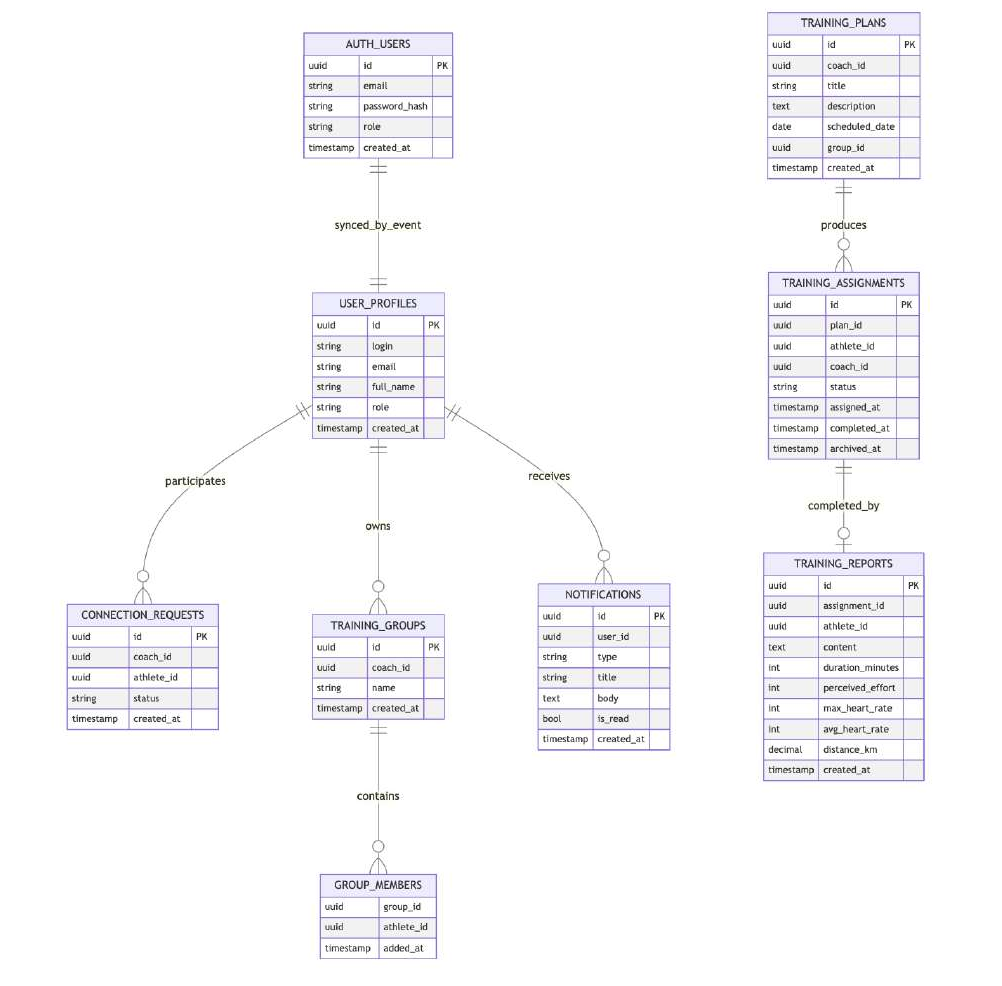
\includegraphics[width=\textwidth]{inc/er-main-tables_cropped.pdf}
  \caption{Расширенная ER-диаграмма основных таблиц платформы CoachLink}
  \label{fig:er-main-tables}
\end{figure}


\appendixsection{События NATS JetStream в backend-платформе}

В приложении приведена таблица событий, используемых для слабосвязанного взаимодействия сервисов.

\begingroup
\TableFontPt{12}
\begin{longtable}{|
  >{\raggedright\arraybackslash}p{0.42\columnwidth}|
  >{\raggedright\arraybackslash}p{0.13\columnwidth}|
  >{\raggedright\arraybackslash}p{0.16\columnwidth}|
  >{\raggedright\arraybackslash}p{0.17\columnwidth}|}
\caption{События NATS JetStream для межсервисного взаимодействия}\label{tab:appendix-nats-events}\\
\hline
\begin{minipage}[b]{\linewidth}\raggedright
Событие
\end{minipage} & \begin{minipage}[b]{\linewidth}\raggedright
Источник
\end{minipage} & \begin{minipage}[b]{\linewidth}\raggedright
Получатель
\end{minipage} & \begin{minipage}[b]{\linewidth}\raggedright
Назначение
\end{minipage} \\
\hline
\endhead
\hline
\endlastfoot
\path|coachlink.user.registered| & Auth Service & User Service & Создание профиля пользователя \\ \hline
\path|coachlink.connection.requested| & User Service & Notification Service & Уведомление тренера о новой заявке \\ \hline
\path|coachlink.connection.accepted| & User Service & Notification Service & Уведомление спортсмена о принятии заявки \\ \hline
\path|coachlink.connection.rejected| & User Service & Notification Service & Уведомление спортсмена об отклонении заявки \\ \hline
\path|coachlink.group.athlete_added| & User Service & Notification Service & Уведомление о добавлении в группу \\ \hline
\path|coachlink.group.athlete_removed| & User Service & Notification Service & Уведомление об удалении из группы \\ \hline
\path|coachlink.training.assigned| & Training Service & Notification Service & Уведомление о назначенной тренировке \\ \hline
\path|coachlink.training.deleted| & Training Service & Notification Service & Уведомление об удалении назначения \\ \hline
\path|coachlink.report.submitted| & Training Service & Notification Service & Уведомление тренера о новом отчёте \\ \hline
\end{longtable}
\endgroup

Названия событий взяты из общего пакета \passthrough{\lstinline!pkg/events!} и соответствуют текущей событийной модели платформы.

\appendixsection{Таблица тестирования}

Таблица тестирования отражает фактически подтверждённые результаты запусков.

\begingroup
\TableFontPt{12}
\begin{longtable}{|
  >{\raggedright\arraybackslash}p{0.23\columnwidth}|
  >{\raggedright\arraybackslash}p{0.24\columnwidth}|
  >{\raggedright\arraybackslash}p{0.22\columnwidth}|
  >{\raggedright\arraybackslash}p{0.19\columnwidth}|}
\caption{Уровни тестирования и критерии фиксации результатов}\label{tab:appendix-test-plan}\\
\hline
\begin{minipage}[b]{\linewidth}\raggedright
Уровень тестирования
\end{minipage} & \begin{minipage}[b]{\linewidth}\raggedright
Команда
\end{minipage} & \begin{minipage}[b]{\linewidth}\raggedright
Назначение
\end{minipage} & \begin{minipage}[b]{\linewidth}\raggedright
Статус
\end{minipage} \\
\hline
\endhead
\hline
\endlastfoot
Unit-тесты & make test-unit & Проверка сервисного слоя отдельных микросервисов & 112 тестов пройдено \\ \hline
E2E smoke & make test-e2e & Проверка базового e2e-сценария при поднятой платформе & 19 шагов пройдено \\ \hline
Integration & make\linebreak test-integration & Проверка API Gateway и межсервисных сценариев & 113 проверок пройдено \\ \hline
\end{longtable}
\endgroup
\end{document}
